%% 11/23/2015
%%%%%%%%%%%%%%%%%%%%%%%%%%%%%%%%%%%%%%%%%%%%%%%%%%%%%%%%%%%%%%%%%%%%%%%%%%%%
% AGUJournalTemplate.tex: this template file is for articles formatted with LaTeX
%
% This file includes commands and instructions
% given in the order necessary to produce a final output that will
% satisfy AGU requirements. 
%
% You may copy this file and give it your
% article name, and enter your text.
%
%%%%%%%%%%%%%%%%%%%%%%%%%%%%%%%%%%%%%%%%%%%%%%%%%%%%%%%%%%%%%%%%%%%%%%%%%%%%
% PLEASE DO NOT USE YOUR OWN MACROS
% DO NOT USE \newcommand, \renewcommand, or \def, etc.
%
% FOR FIGURES, DO NOT USE \psfrag or \subfigure.
% DO NOT USE \psfrag or \subfigure commands.
%%%%%%%%%%%%%%%%%%%%%%%%%%%%%%%%%%%%%%%%%%%%%%%%%%%%%%%%%%%%%%%%%%%%%%%%%%%%
%
% All questions should be e-mailed to latex@agu.org.
%
%%%%%%%%%%%%%%%%%%%%%%%%%%%%%%%%%%%%%%%%%%%%%%%%%%%%%%%%%%%%%%%%%%%%%%%%%%%%
%
% Step 1: Set the \documentclass
%
% There are two options for article format:
%
% 1) PLEASE USE THE DRAFT OPTION TO SUBMIT YOUR PAPERS.
% The draft option produces double spaced output.
% 
% 2) numberline will give you line numbers.

%% To submit your paper:

\documentclass[draft,linenumbers]{agujournal}
\drafttrue
\usepackage{graphicx, xcolor}

%% For final version.
% \documentclass{agujournal}

% Now, type in the journal name: \journalname{<Journal Name>}

% ie, \journalname{Journal of Geophysical Research}
%% Choose from this list of Journals:
%
% JGR-Atmospheres
% JGR-Biogeosciences
% JGR-Earth Surface
% JGR-Oceans
% JGR-Planets
% JGR-Solid Earth
% JGR-Space Physics
% Global Biochemical Cycles
% Geophysical Research Letters
% Paleoceanography
% Radio Science
% Reviews of Geophysics
% Tectonics
% Space Weather
% Water Resource Research
% Geochemistry, Geophysics, Geosystems
% Journal of Advances in Modeling Earth Systems (JAMES)
% Earth's Future
% Earth and Space Science
%
%

\journalname{JGR-Biogeosciences}


\begin{document}

%% ------------------------------------------------------------------------ %%
%  Title
% 
% (A title should be specific, informative, and brief. Use
% abbreviations only if they are defined in the abstract. Titles that
% start with general keywords then specific terms are optimized in
% searches)
%
%% ------------------------------------------------------------------------ %%

% Example: \title{This is a test title}

\title{{\color{blue}Understanding the effect of disturbance on the carbon dynamics of a managed woodland}}

%% ------------------------------------------------------------------------ %%
%
%  AUTHORS AND AFFILIATIONS
%
%% ------------------------------------------------------------------------ %%

% Authors are individuals who have significantly contributed to the
% research and preparation of the article. Group authors are allowed, if
% each author in the group is separately identified in an appendix.)

% List authors by first name or initial followed by last name and
% separated by commas. Use \affil{} to number affiliations, and
% \thanks{} for author notes.  
% Additional author notes should be indicated with \thanks{} (for
% example, for current addresses). 

% Example: \authors{A. B. Author\affil{1}\thanks{Current address, Antartica}, B. C. Author\affil{2,3}, and D. E.
% Author\affil{3,4}\thanks{Also funded by Monsanto.}}

\authors{Ewan M. Pinnington\affil{1}, Eric Casella\affil{3}, Sarah L. Dance\affil{1,2}, Amos S. Lawless\affil{1,2,4}, James I. L. Morison\affil{3}, Nancy K. Nichols\affil{1,2,4}, Matthew Wilkinson\affil{3}, Tristan L. Quaife\affil{1,4}}


% \affiliation{1}{First Affiliation}
% \affiliation{2}{Second Affiliation}
% \affiliation{3}{Third Affiliation}
% \affiliation{4}{Fourth Affiliation}

\affiliation{1}{Department of Meteorology, University of Reading, Reading, UK}
\affiliation{2}{Department of Mathematics and Statistics, University of Reading, Reading, UK}
\affiliation{3}{Centre for Sustainable Forestry and Climate Change, Forest Research, Alice Holt, Farnham, UK}
\affiliation{4}{National Centre for Earth Observation, University of Reading, Reading, UK}

%(repeat as many times as is necessary)

%% Corresponding Author:
% Corresponding author mailing address and e-mail address:

% (include name and email addresses of the corresponding author.  More
% than one corresponding author is allowed in this LaTeX file and for
% publication; but only one corresponding author is allowed in our
% editorial system.)  

% Example: \correspondingauthor{First and Last Name}{email@address.edu}

\correspondingauthor{Ewan M. Pinnington}{e.m.pinnington@pgr.reading.ac.uk}

%% Keypoints, final entry on title page.

% Example: 
% \begin{keypoints}
% \item	List up to three key points (at least one is required)
% \item	Key Points summarize the main points and conclusions of the article
% \item	Each must be 100 characters or less with no special characters or punctuation 
% \end{keypoints}

%  List up to three key points (at least one is required)
%  Key Points summarize the main points and conclusions of the article
%  Each must be 100 characters or less with no special characters or punctuation 

\begin{keypoints}
\item {\color{blue}No change was found in NEE after selective felling}
\item Data assimilation was used to investigate the effect of this disturbance 
\item {\color{blue}Concurrent reductions in respiration and GPP allow for unchanged NEE}
\end{keypoints}

%% ------------------------------------------------------------------------ %%
%
%  ABSTRACT
%
% A good abstract will begin with a short description of the problem
% being addressed, briefly describe the new data or analyses, then
% briefly states the main conclusion(s) and how they are supported and
% uncertainties. 
%% ------------------------------------------------------------------------ %%

%% \begin{abstract} starts the second page 

\begin{abstract}
The response of forests and terrestrial ecosystems to disturbance is an important process in the global carbon cycle in the context of a changing climate. {\color{blue}(1)This study focuses on the effect of selective felling (thinning) at a managed forest site. Previous statistical analyses of eddy covariance data at the study site had found that disturbance from thinning resulted in no significant change to the net carbon uptake of the ecosystem. In order to better understand possible explanations for this observation we use the mathematical technique of data assimilation to combine a diverse set of data with a mathematical model of ecosystem carbon balance. Data assimilation provides a compelling alternative to more common statistical analyses of flux data as it allows for the combination of many different sources of data to find an improved estimate to the state of a system.} We develop {\color{blue} new observation operators} allowing for the assimilation of daytime and nighttime net ecosystem exchange observations with a daily time-step model, increasing {\color{blue}observations} available by a factor of 4.25. These techniques allow us to estimate the effect of step-changes in ecosystem composition on the parameter and state variables in a {\color{blue}modeled} estimate of forest carbon balance. These techniques are applicable to other ecosystem models and data assimilation schemes. 

Our results support previous analyses, with a predicted net ecosystem carbon uptake for the year 2015 of \(426 \pm 116~\text{g C m}^{-2}\) for the unthinned forest and \(420 \pm 78~\text{g C m}^{-2}\) for the thinned forest despite a model-predicted reduction in gross primary productivity of \(337~\text{g C m}^{-2}\). We show that this is likely due to reduced ecosystem respiration post-disturbance compensating for a reduction in gross primary productivity. This supports the theory of an upper limit of forest net carbon uptake due to the magnitude of ecosystem respiration scaling with gross primary productivity.  \end{abstract}


%% ------------------------------------------------------------------------ %%
%
%  TEXT
%
%% ------------------------------------------------------------------------ %%

%%% Suggested section heads:
% \section{Introduction}
% 
% The main text should start with an introduction. Except for short
% manuscripts (such as comments and replies), the text should be divided
% into sections, each with its own heading. 

% Headings should be sentence fragments and do not begin with a
% lowercase letter or number. Examples of good headings are:

% \section{Materials and Methods}
% Here is text on Materials and Methods.
%
% \subsection{A descriptive heading about methods}
% More about Methods.
% 
% \section{Data} (Or section title might be a descriptive heading about data)
% 
% \section{Results} (Or section title might be a descriptive heading about the
% results)
% 
% \section{Conclusions}


\section{Introduction}
%Disturbance can take many forms, for example; felling, fire and insect outbreak. In current estimates of the global carbon budget, disturbance is one of the least understood components. In this paper, we investigate the effect of the management practice f selective felling on the carbon dynamics of a mature temperate woodland.

%\subsection{\textcolor{red}{Role of disturbance in the global C cycle (make flow better?)}}
The response of forests and terrestrial ecosystems to disturbance (e.g. felling, fire, or insect outbreaks) is one of the least understood components in the global carbon cycle \citep{ciais2014carbon}. Current land surface models fail to represent the effect of disturbances on long-term carbon dynamics \citep{running2008ecosystem}, although these disturbances could have a significant effect on net land surface carbon uptake. Indeed, there could be significant variations in the effect as the range of forest disturbance can be wide: from {\color{blue}stand-replacing} disturbance (where tree mortality is close to 100\%) to non-{\color{blue}stand-replacing} disturbance, (where only a proportion of trees are lost). This paper uses data assimilation to improve the modelling of the non-{\color{blue}stand-replacing} disturbance of selective felling (thinning) on forest carbon dynamics.

%\subsection{\textcolor{red}{Current theories on terrestrial ecosystem response to disturbance}}
Thinning is a silvicultural practice used to improve ecosystem services or the quality of a final tree crop and is globally widespread. The effect of thinning on carbon budgets has largely been ignored \citep{JGRG:JGRG779}. {\color{blue}Thinning has been shown to increase the basal growth increment of remaining trees due to increased light and water availability \citep{breda95thin, martin2010response}. \citet{Misson2005207} found that the immediate effect of thinning can change an ecosystem from a sink to a source of CO$_{2}$, due to reduced Gross Primary Productivity (GPP) following a reduction in total leaf area and unchanged or heightened ecosystem respiration}. However, other studies, analysing flux-tower eddy covariance records, find no significant change in the observed net ecosystem exchange (NEE) of CO\(_{2}\) after thinning \citep{vesala2005effect, moreaux2011paired,  dore2012recovery, Saunders20121, wilkinson2015effects}. These studies suggest this is due to increased light availability and reduced competition allowing ground vegetation to display increased GPP and compensate for an increase in heterotrophic respiration post-disturbance.  

Other studies have shown a significant reduction in the carbon content of rhizosphere soils following tree felling \citep{Hernesmaa2005777}. It has been shown that tree roots provide a rhizosphere priming effect, greatly increasing the rate of soil organic carbon decomposition \citep{ELE:ELE1095}. This is consistent with previous work carried out at the study site in this paper, where it has been shown that the magnitude of ecosystem respiration is strongly coupled to the magnitude of GPP \citep{heinemeyer2012exploring}. Predictions made by \citet{kurz2008mountain} about the impacts of mountain pine beetle outbreaks in Northern American forests suggested a switch from sink to source of carbon following this disturbance. However, the analysis of a diverse set of observations for an area with approximately 70\% infested trees by \citet{ELE:ELE12097} revealed little change in net CO\(_{2}\) flux, due to concurrent reductions in GPP and ecosystem respiration. Similar results were also found from large scale tree girdling experiments \citep{hogberg2001large}, where 1-2 months after girdling a 54\% decrease in soil respiration was observed.

%\subsection{\textcolor{red}{The role of data assimilation for improving estimates to a system}}
Here we used data assimilation{\color{blue},} which is a mathematical technique for combining observations with prior model predictions in order to find the best estimate of a dynamical system. Functional ecology models have been combined with many different observations relevant to the carbon balance of forests \citep{Quaife2008, fox2009reflex, zobitz2011primer, richardson2010estimating, Zobitz2014, Niu2014, Pinnington2016299}, leading to improved estimates of model parameter and state variables and reduced uncertainty in model predictions. There have been many efforts to model the effect of disturbance on forest ecosystems \citep{thornton2002modeling, seidl2011modelling}, {\color{blue}with a growing number of dynamic global vegetation models \citep{sitch2008evaluation}}. However, the use of data assimilation has been limited to a few examples, all of which used satellite data \citep{hilker2009new, kantzas2015improving}. The authors are not aware of any studies assimilating site level data to quantify disturbance effects. By assimilating observations relevant to post-disturbance ecosystem carbon dynamics with prior model predictions of ecosystem behaviour, we can analyse the retrieved parameters after data assimilation to find the model predicted effects of disturbance.   

%\subsection{\textcolor{red}{What does this paper do?}}
In this paper we investigate the effect of thinning on the carbon dynamics of the Alice Holt flux site \citep{wilkinson2012inter}, a deciduous managed woodland, following an event in 2014, when one side of the site was thinned and the other side left unmanaged. 
%During this thinning approximately 46\% of trees were removed from the studied area. In order to better understand the effect this thinning had on stand structure an intensive field campaign was undertaken in 2015 to measure leaf area index and also estimate woody biomass for both sides of the study site. The site has a flux tower positioned on the boundary between the thinned and unthinned forest. The eddy covariance record of NEE was split between the two sides using a flux footprint model. Previous statistical analysis of a thinning event in 2007 had suggested that there was no change in NEE between the thinned and unthinned sides of the forest post-disturbance \citep{wilkinson2015effects}.  
We present new methods for the assimilation of daytime and nighttime NEE observations with a daily time-step model, in this case the Data Assimilation Linked Ecosystem Carbon (DALEC2) model \citep{Bloom2015}. These methods require no model modification. We combine all available observations for 2015 with prior model predictions to find two sets of optimised model parameter and initial state values, corresponding to thinned and unthinned sides of the forest. We then use these two versions of the model to seek to explain why the net uptake of carbon remains unchanged even after removing a large proportion of the trees from one side. We find a net ecosystem carbon uptake for the year 2015 of \(426 \pm 116~\text{g C m}^{-2}\) for the unthinned forest and \(420 \pm 78~\text{g C m}^{-2}\) for the thinned forest, despite a reduction in GPP of \(337~\text{g C m}^{-2}\) for the thinned forest when compared to the unthinned forest. We find that reduced ecosystem respiration for the thinned forest allows for this unchanged net carbon uptake. The data assimilation techniques presented in this paper could be applied for similar analyses at other sites and provide a novel method to help elucidate the reasons behind ecosystem responses.      

\section{Observation and data assimilation methods}

\subsection{Alice Holt research forest} \label{sec:site_description}

Alice Holt Forest is a research forest area managed by the UK Forestry Commission located in Hampshire, SE England. Forest Research has been operating a $\text{CO}_{2}$ flux measurement tower in a portion of the forest, the Straits Inclosure, continuously since 1998. The Straits Inclosure is a $90~\text{ha}$ area of deciduous broadleaved plantation woodland located on a surface water gley soil and has been managed for the past 80 years. The majority of the canopy trees are oak (\textit{Quercus robur} L.), with an understory of hazel (\textit{Corylus avellana} L.) and hawthorn (\textit{Crataegus monogyna} Jacq.), but there is a small area of conifers (\textit{Pinus nigra} ssp. \textit{laricio} (Maire) and \textit{P. sylvestris} L.) within the tower measurement footprint area depending on wind direction. Further details of the Straits Inclosure site and the measurement procedures are given in \citet{wilkinson2012inter}, together with analysis of stand-scale $30$ minute average net $\text{CO}_{2}$ fluxes (NEE) from 1998-2011. 

As part of the management regime, the Straits Inclosure is subject to thinning, whereby a proportion of trees are removed from the canopy in order to reduce competition and improve the quality of the final tree crop. At the Straits an intermediate thinning method is used with a portion of both subdominant and dominant trees being removed from the stand {\color{blue}to stimulate the growth of remaining dominant trees} \citep{kerr2011thinning}. The whole of the stand was thinned in 1995. Subsequently the eastern side of the Straits was thinned in 2007 and then the western side in 2014. The flux tower at the site is situated on the boundary between these two sides. This allows for the use of a footprint model to split the flux record and thus analyse the effect of this disturbance on carbon fluxes at the site. In \citet{wilkinson2015effects} a statistical analysis of the eddy covariance flux record found that there was no significant effect on the net carbon uptake of the eastern side after thinning in 2007. In this paper we focus on the effect of disturbance on the western side after thinning in 2014. We therefore refer to the western side as ``thinned'' forest and the eastern side as ``unthinned'' forest, {\color{blue}although the ``unthinned'' forest was previously thinned in 2007 and so will have a different structure to a completely unmanaged forest}.   

\subsection{Observations} \label{sec:obs}

In order to assess the effect the 2014 thinning had on the Straits Inclosure, an intensive field campaign was undertaken in 2015 to measure leaf area index and also to estimate standing woody biomass. From the site we also have a long record of flux data, as discussed in section~\ref{sec:site_description}. These observations span both the thinned and unthinned sides of the forest.

\subsubsection{Leaf area index}

To assess the impact of the 2014 thinning, three transects were established in the Straits Inclosure for intensive sampling during 2015. A total of 435 sampling points were marked at 10~m apart, using a GPS and fluorescent tree spray paint. Measurements of peak LAI (July 2015 - September 2015) were made using both a ceptometer and hemispherical photography. The transects were walked twice with the ceptometer taking readings at every sampling point, giving 870 readings in total. Hemispherical photographs were taken every 50~m as shown in Figure~\ref{fig:hemi_lai}, giving 89 photographs in total. 

We measured below-canopy Photosynthetically Active Radiation (PAR) using the ceptometer while logging above-canopy PAR using a data logger and PAR sensor positioned outside the canopy. We then estimated LAI using the above-canopy and below-canopy PAR readings \citep{fassnacht1994comparison}. For the hemispherical photographs, we used the HemiView software \citep{rich1999hemiview} which calculates the proportion of visible sky as a function of sky direction (gap fraction) which it then uses to calculate LAI \citep{Jonckheere2004}.

Six litter traps were also established at points along the transects (positions shown in Figure~\ref{fig:hemi_lai}) allowing for comparison with the other methods. These were sampled throughout the leaf-fall season in 2015. We found the LAI derived from the litter traps was always greater than LAI estimated from optical methods, as expected \citep{breda2003ground}. From the sampling of the litter traps we also have estimates of {\color{blue}leaf mass per leaf area} for use in data assimilation. As the 6 litter traps are not enough to describe the LAI for the research site \citep{kimmins1973some}, we used estimates from the ceptometer and hemispherical photographs for data assimilation. We took the weighted average (dependent on number of observations taken of each type) of the hemispherical photograph and ceptometer estimated LAI and derived an LAI of 4.42 with a standard error of 0.07 for the eastern unthinned forest, and an LAI of 3.06 with a standard error of 0.07 for the western thinned forest. We assimilated the mean of 299 LAI observations in the unthinned and 225 in the thinned section of forest. Consequently the appropriate representation of error for data assimilation is the standard error of the mean. From our litter trap observations we find a leaf mass per area of 29~g~C~m\(^{-2}\) free soluble carbohydrates for both sides of the forest.


\begin{figure}[ht]
    \centering
    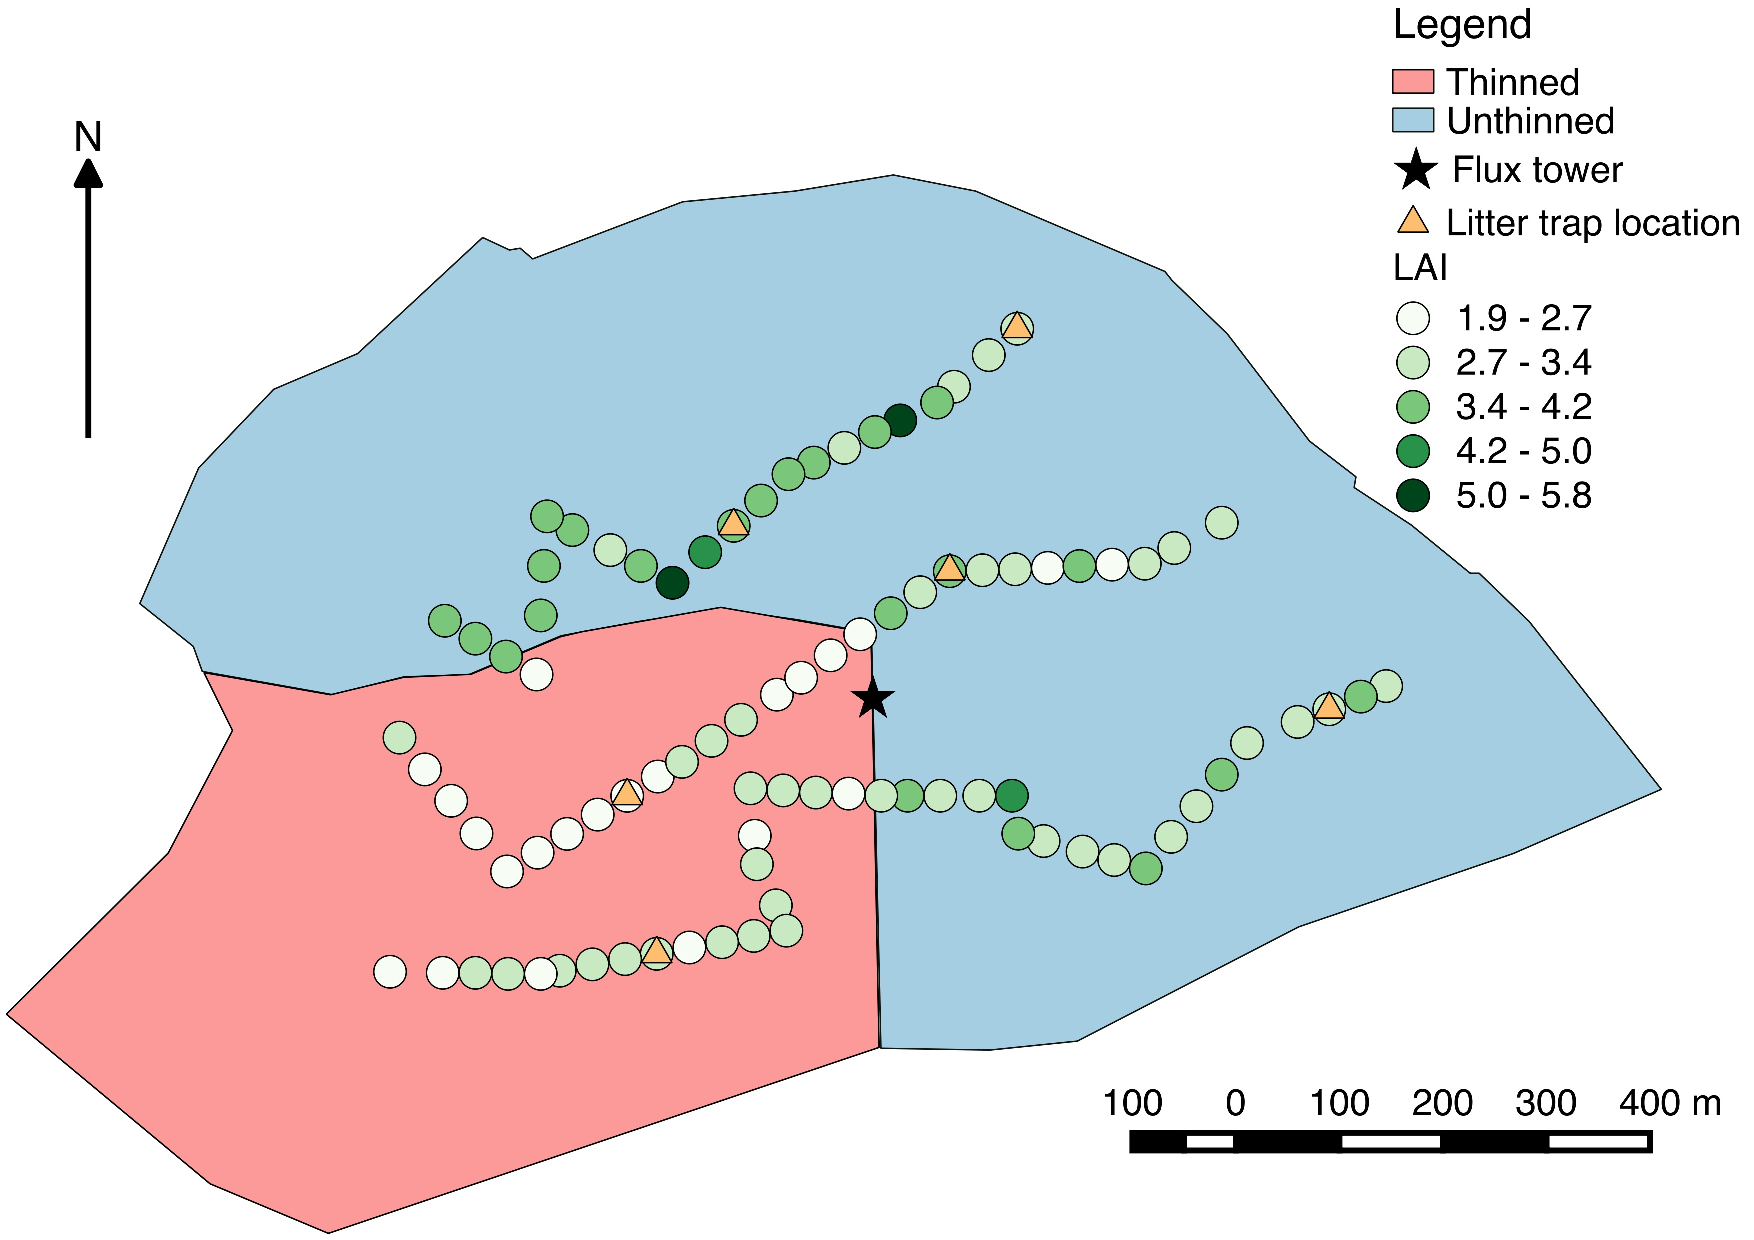
\includegraphics[width=0.8\textwidth]{thinned.pdf}
    \caption{LAI derived from hemispherical photographs for the Straits Inclosure at 50m intervals along three transects.} \label{fig:hemi_lai}
\end{figure}

\subsubsection{Woody biomass}  
The method of Point-Centred Quarters (PCQ) was used to conduct a biomass survey as specified in \citet{dahdouh2006empirical}. Along the three transects 114 points were sampled measuring the Diameter at Breast Height (DBH) and the density of trees. We then used allometric relationships between DBH and total above ground biomass and coarse root biomass, found in work carried out by Forest Research and in \citet{mckay2003woodfuel}, to find an estimate of total woody and coarse root carbon (referred to as \(C_{woo}\) in the DALEC2 model). These observations are shown in table~\ref{table:cwoo_obs}.

Forest Research have carried out their own mensuration studies at the site. One such study of the western thinned forest (at a similar time to our own PCQ measurements) found a tree density of 225 ha\(^{-1}\) and an average DBH of 32 cm, which are in close agreement to the estimates in table~\ref{table:cwoo_obs}. This gives us confidence that earlier measurements taken by Forest Research before the thinning are representative of the methods we have used. Measurements of the same section of forest from 2009 found a tree density of 418 ha\(^{-1}\) and an average DBH of 28 cm. This suggests that approximately 46\% of trees have been removed during the 2014 thinning. From these estimates we can also see the effect thinning has on the type of trees found at the site. The trees per hectare has dropped dramatically after thinning but the mean DBH has increased, because the smaller subdominant trees have been removed. The greater mean DBH of the eastern unthinned section, \(34~\text{cm}\), indicates that the thinning that took place in 2007 has allowed the dominant trees to grow as a result of reduced competition.

\begin{table}[ht] 
	\caption{Point-centred quarter method observations for 2015.}
\begin{center}
	\begin{tabular}{| l | p{2cm} | p{2cm} | p{4.5cm} |}
	\hline
	Sector & Tree density (ha\(^{-1}\)) & Mean DBH (cm) & Estimated woody biomass and coarse root carbon (g C m\(^{-2}\)) \\ \hline
	Unthinned (E) & 272 & 34.12 & 13130 \\ \hline
	Thinned (W) & 225 & 32.85 & 9908 \\ \hline
	\end{tabular}
	\label{table:cwoo_obs}
\end{center} 
\end{table}

\subsubsection{Flux tower eddy covariance} \label{sec:eddycov} 

The Straits Inclosure flux tower provides half-hourly observations from January 1999 to December 2015. These consist of the NEE fluxes and meteorological driving data of temperature, irradiance and atmospheric CO\(_{2}\) concentration for use in the DALEC2 model. The NEE data was subject to \(u^*\) filtering (with a value of \(0.2~\text{m s}^{-1}\)) and quality control procedures as described by \citet{papale2006towards}, but was not gap-filled. The resultant half-hourly NEE dataset was then split between observations corresponding to the western thinned and eastern unthinned sides of the site using a flux-footprint model, see \citet{wilkinson2015effects} for more details.  

To match the time-step of our model we computed daily NEE observations by taking the mean over the 48 measurements made each day, selecting only days where there is no missing data. As we have been strict on the quality control of the flux record and not used any gap filling, this presented a problem in terms of the number of daily NEE observations available. By further splitting the flux record between two sides we retrieved very few total daily observations of NEE for either side. In order to address this we computed day and nighttime NEE fluxes (NEE\(_{day}\) and NEE\(_{night}\) respectively) for use in data assimilation. We used a solar model to define whether NEE measurements were made at daytime or nighttime. We then took the mean over the half-hourly day or nighttime measurements, again only taking periods where there were no gaps in the data so that we were only considering true observations. This provided us with many more observations of NEE for assimilation, as seen in table~\ref{table:nee_obs}. Because we are averaging over shorter time periods we have a smaller probability of gaps and erroneous data. We see that we have more daytime NEE observations than nighttime, as we tend to have much more turbulent air mixing in daylight hours. In section~\ref{sec:da} we give details of how we relate these twice daily observations of NEE to a daily time-step model.     

\begin{table}[ht] 
	\caption{Number of observations of NEE, NEE\(_{day}\) and NEE\(_{night}\) for East and West sides of the Straits Inclosure for the year 2015.}
\begin{center}
	\begin{tabular}{| l | l | l | l | l |}
	\hline
	Sector & NEE & NEE\(_{day}\) & NEE\(_{night}\)  \\ \hline
	Unthinned (E) & 22 & 60 & 42 \\ \hline
	Thinned (W) & 26 & 54 & 48 \\ \hline
	\end{tabular}
	\label{table:nee_obs}
\end{center} 
\end{table}

The errors in observations of daily NEE were assumed to be constant and set at $0.5~\text{g C m}^{-2} \text{day}^{-1}$ by \citet{williams2005improved}, whereas \citet{braswell2005estimating} found these errors to be closer to $1~\text{g C m}^{-2} \text{day}^{-1}$. However, \citet{Richardson200838} show that flux errors are heteroscedastic. To account for the heteroscedastic nature of NEE errors we define an error function that scales between $0.5$ to $1~\text{g C m}^{-2} \text{day}^{-1}$ based on the magnitude of the observation. This function is defined as $0.5 + 0.04|\text{NEE}_{\text{day}}^{i}|~\text{g C m}^{-2} \text{day}^{-1}$, where \(|\text{NEE}_{\text{day}}^{i}|\) is the magnitude of the daytime NEE observation. \citet{raupach2005model} comment that nighttime measurements of NEE are much more uncertain than daytime measurements. This is difficult to quantify, but here we assume that nighttime flux errors are 3 times the magnitude of daytime errors. We therefore have the error function of $1.5 + 0.12|\text{NEE}_{\text{night}}^{i}|~\text{g C m}^{-2} \text{day}^{-1}$, where \(|\text{NEE}_{\text{night}}^{i}|\) is the magnitude of the nighttime NEE observation. We also include correlations in time between the errors in our observations of NEE, as discussed in \citet{Pinnington2016299}.

\subsection{Model and data assimilation}
\subsubsection{DALEC2 ecosystem carbon model} \label{sec:dalec2}

The DALEC2 model is a simple process-based model describing the carbon dynamics of a forest ecosystem \citep{Bloom2015}. The model is constructed of six carbon pools (labile ($C_{lab}$), foliage ($C_{fol}$), fine roots ($C_{roo}$), woody stems and coarse roots ($C_{woo}$), fresh leaf and fine root litter ($C_{lit}$) and soil organic matter and coarse woody debris ($C_{som}$)) linked via fluxes. The aggregated canopy model (ACM) \citep{williams1997predicting} is used to calculate daily gross primary production ($GPP$) of the forest, taking meteorological driving data and the {\color{blue}modeled} leaf area index (a function of $C_{fol}$) as arguments. Figure~\ref{fig:DALEC_mod} shows a schematic of how the carbon pools are linked in DALEC2; full model equations can be found in the appendix, section \ref{sec:dalec_eqns}.   

\begin{figure}[ht]
    \centering
    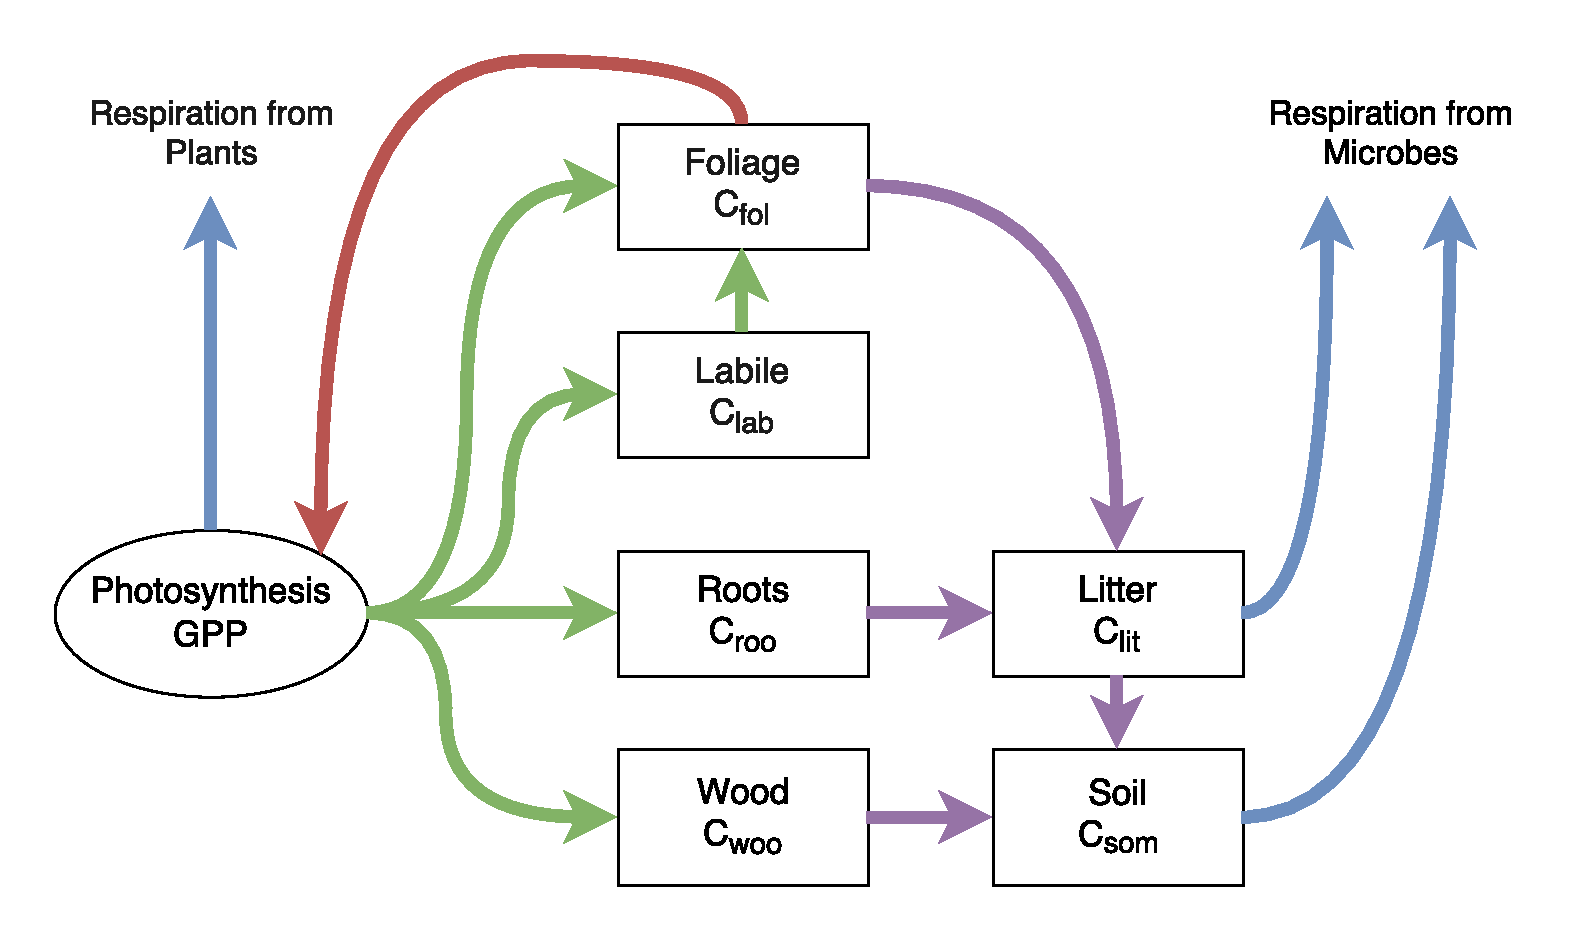
\includegraphics[width=0.6\textwidth]{dalec2diag.pdf}
    \caption{Representation of the fluxes in the DALEC2 carbon balance model. Green arrows represent C allocation, purple arrows represent litter fall and decomposition fluxes, blue arrows represent respiration fluxes and the red arrow represents the influence of leaf area index in the $GPP$ function.} \label{fig:DALEC_mod}
\end{figure}

\subsubsection{Data assimilation} \label{sec:da}

We implement Four-Dimensional Variational data assimilation (4D-Var) with the DALEC2 model for joint parameter and state estimation \citep{navon1998practical}. In 4D-Var we aim to find the parameter and initial state values such that the model trajectory best fits the data over some time window, given some prior information about the system. This prior information takes the form of an initial estimate of the parameter and state variables of the model, $\textbf{x}^{b}$, valid at the initial time. This prior is assumed to have unbiased, Gaussian errors with known covariance matrix $\textbf{B}$. Adding the prior term ensures that our problem is well posed and that we can find a locally unique solution \citep{Tremolet2006}. We aim to find the parameter and initial state values that minimise the weighted squared distance to the prior and the weighted squared distance of the model trajectory to the observations, over a time window of length \(N\), with individual time points $t_{0}, \dots, t_{N}$. We do this by finding the state $\textbf{x}^{a}$ at time $t_{0}$ that minimises the cost function

\begin{linenomath*}
\begin{equation}
J(\textbf{x}_0) = \frac{1}{2}(\textbf{x}_0-\textbf{x}^b)^{T}\textbf{B}^{-1}(\textbf{x}_0-\textbf{x}^b)+\frac{1}{2}\sum_{i=0}^{N}(\textbf{y}_i-\textbf{h}_i(\textbf{x}_i))^{T}\textbf{R}_{i}^{-1}(\textbf{y}_i-\textbf{h}_i(\textbf{x}_i)),
\end{equation}
\end{linenomath*}
where $\textbf{x}_{0}$ is the vector of parameter and initial state values to be optimised, $\textbf{x}_{i}$ is the vector of model variables at time \(t_{i}\), $\textbf{h}_{i}$ is the observation operator mapping the parameter and state values to the observations, $\textbf{y}_{i}$ is the vector of observations at time \(t_i\) and $\textbf{R}_{i}$ is the observation error covariance matrix. The time step, \(i\), is 1 day in this case. Further details of the implemented data assimilation scheme and specification of prior and observational errors can be found in \citet{Pinnington2016299}. 

In this paper we assimilate day and nighttime NEE in order to increase the number of observations available to us and also better partition our {\color{blue}modeled} estimate of GPP and total ecosystem respiration. As the DALEC2 model runs at a daily time step, this requires us to relate the daily parameter and state values from the model to the twice-daily observations of NEE. We do this by writing two new observation operators, one relating the model state and parameters to daytime NEE, and the other to nighttime NEE. The NEE of CO\(_{2}\) at any given time is the difference between GPP and ecosystem respiration. For an observation of total daily NEE on day \(i\) we have,
\begin{linenomath*}
\begin{equation}
NEE^{i}=-GPP^{i}(C_{fol}^{i}, \Psi) +f_{auto}GPP^{i}(C_{fol}^{i}, \Psi) + \theta_{lit}C_{lit}^i e^{\Theta T^{i}} + \theta_{som}C_{som}^i e^{\Theta T^{i}}, \label{eqn: D1_nee}
\end{equation}
\end{linenomath*}
where \(\Psi\) represents meteorological driving data used the in the calculation of GPP, \(f_{auto}\) is the fraction of autotrophic respiration, \(\theta_{lit}\) is the litter carbon turnover rate, \(\theta_{som}\) is the soil and organic carbon turnover rate, \(\Theta\) is the temperature dependence exponent factor and \(T^{i}\) is the mean temperature over 24~hours. Further description can be found in the appendix section~\ref{sec:dalec_eqns}. The first term in equation~\eqref{eqn: D1_nee} represents gross primary productivity, the second autotrophic respiration and the third and fourth terms heterotrophic respiration. 

For total daytime NEE we have,
\begin{linenomath*}
\begin{equation}
NEE_{day}^{i} = -GPP^{i}(C_{fol}^{i}, \Psi) + \delta_{day}f_{auto}GPP^{i}(C_{fol}^{i}, \Psi) + \delta_{day}\theta_{lit}C_{lit}^i e^{\Theta T_{day}^{i}} + \delta_{day}\theta_{som}C_{som}^i e^{\Theta T_{day}^{i}} \label{eqn: D1_nee_day}
\end{equation}
\end{linenomath*}
where \(\delta_{day}\) is \(\frac{\text{number of daylight hours}}{24}\), and \(T_{day}^{i}\) is the mean temperature over daylight hours. Here we still have the same term for GPP as in equation~\eqref{eqn: D1_nee} as all photosynthesis occurs during daylight hours. We have made the assumption that respiration is spread uniformly in time; therefore the respiration terms are scaled by the fraction of daylight hours. For nighttime NEE we have,
\begin{linenomath*}
\begin{equation}
NEE_{night}^{i} =  \delta_{night}f_{auto}GPP^{i}(C_{fol}^{i}, \Psi) + \delta_{night}\theta_{lit}C_{lit}^i e^{\Theta T_{night}^{i}} + \delta_{night}\theta_{som}C_{som}^i e^{\Theta T_{night}^{i}} \label{eqn: D1_nee_night}
\end{equation}
\end{linenomath*}
where \(\delta_{night}\) is \(\frac{\text{number of night hours}}{24}\), and \(T_{night}^{i}\) is the mean nighttime temperature. In equation~\eqref{eqn: D1_nee} we do not have a term for GPP as no GPP will occur during the night. The respiration is here is scaled by the fraction of nighttime hours. The length of day and night are calculated using a solar model.

 These new observation operators allow for assimilation of day/nighttime NEE without the need for altering the model and can be applied to other ecosystem models to allow for the assimilation of eddy covariance data at a finer temporal resolution. 
%Cite MacBean?? for correlations?

\subsection{Experimental setup}
%Assimilation of 2015 years data post disturbance for the optimisation of two parameter sets, one corresponding to the unmanaged East and the other set to the managed West.

%In this paper we have split the flux tower eddy covariance record using a footprint model. This means we have observations of NEE for both the West and East sides of the forest stand. By combining these two distinct sets of observations with our prior model using 4D-Var data assimilation allows us to retrieve two unique sets of parameter and initial state values, .

In order to assess the information content of the three available data streams (described in section~\ref{sec:obs}) and their impact on the effect of disturbance as predicted by the model, we conducted a data denial procedure. This involved assimilating different combinations of observations, in three experiments, as shown in table~\ref{table:obs_da}. In our first experiment we used only the eddy covariance data, as this is the data type most commonly used in data assimilation studies. In the second we added the observations relating to leaf mass and area and finally in the third experiment we added the observations of woody biomass, as NEE observations have been shown to be unable to constrain this \citep{fox2009reflex}. In each experiment we used the prior model as specified in the appendix in table~\ref{table:xbvars}. This prior model was found by assimilating daytime and nighttime NEE, leaf mass per area and LAI observations from 2012 and 2013 before the thinning occurred. More information on the methods used to find this prior model can be found in \citet{Pinnington2016299}. 

%We ran three data assimilation experiments for the one year window of 2015. In these experiments we assimilated different combinations of observations as shown in table~\ref{table:obs_da}. By performing this type of ``data denial'' procedure we can assess the relative levels of information from the different data streams and their impact on the disturbance effect predicted by the model. In each experiment we used the prior model as specified in table~\ref{table:xbvars}. This prior model was found by assimilating daytime and nighttime NEE, leaf mass per area and LAI observations from 2012 and 2013 before the thinning occurred. More information on the methods used to find this prior model can be found in \citet{Pinnington2016299}.   

In each experiment we ran the assimilation for both the thinned forest and the unthinned forest, using the distinct data for each side. This allowed us to retrieve a unique set of parameter and initial state values for each section of forest. We analysed the optimised parameter and initial state values for the thinned and unthinned forest and also the model predictions of different variables for each side post-disturbance. This allowed us to judge the effect the thinning in 2014 had on the carbon dynamics of the forest in 2015.

\begin{table}[ht] 
	\caption{Combination of observations used in data assimilation experiments.}
\begin{center}
	\begin{tabular}{| l | l | l | l |}
	\hline
	Experiment & NEE & LAI \& leaf mass per area & C\(_{woo}\) \\ \hline
	A & \(\times\) &  &  \\ \hline
	B & \(\times\) & \(\times\) &  \\ \hline
	C & \(\times\) & \(\times\) & \(\times\)  \\ \hline
	\end{tabular}
	\label{table:obs_da}
\end{center} 
\end{table}

It would be expected that we will retrieve different estimates for each of the experiments outlined in table~\ref{table:obs_da}, with our most confident estimate being when all observations types are assimilated together in experiment C. This would allow us to see how much information each data stream provides and assess whether NEE data alone is enough to understand the effect of disturbance.

\section{Results} \label{sec:results}
%Show plots of East and West after assimilation and the change in optimised parameters. Confident in results as we know that even assimilating a single year of data we can accurately describe the carbon dynamics of the site for a long time period (15 years) into the future from Pinnington et al 2016.

In Figure~\ref{fig:obscompa} and \ref{fig:obscompc} we show the observations and model trajectories after assimilation for the  thinned and unthinned forest for experiments A and C respectively. We can see that the model fits all the assimilated observations well after assimilation for both experiments. We have confidence in our results as we have demonstrated previously that assimilating a single year of data can accurately forecast the carbon uptake of the site for a long time period (15 years) \citep{Pinnington2016299}. From Figure~\ref{fig:obscompa}a and \ref{fig:obscompa}b we see that the modified observation operators presented in section~\ref{sec:da} have allowed our model to represent both daytime and nighttime NEE well. 

In experiment A we have only assimilated NEE observations. From table~\ref{table:mod_rmse} we can see that we improve the fit to the assimilated observations for both the unthinned and thinned forest when compared to the prior model. The root-mean-square error (RMSE) is within the specified observation error for both daytime and nighttime NEE after assimilation. By only assimilating observations of NEE we have not been able to accurately predict LAI. Although we have improved the fit of the model to LAI after assimilation for the thinned forest (see table~\ref{table:mod_rmse}), we have significantly degraded the fit of the model to LAI for the unthinned forest. Partitioning the NEE dataset between the thinned and unthinned forest (as described in section~\ref{sec:eddycov}) has resulted in a gap in the observations for the unthinned forest during the period of greatest carbon uptake (June 2015 - August 2015), see Figure~\ref{fig:obscompa}a. This is due to the prevailing wind in this period being from the south-west. The gap in the NEE dataset when observations would have been of highest magnitude causes our model to under-predict the carbon uptake for the unthinned forest. This bias introduced into the NEE dataset for the unthinned forest results in a {\color{blue}significant} under-prediction of LAI, as seen in Figure~\ref{fig:obscompa}c. From Figure~\ref{fig:obscompa}d and table~\ref{table:mod_rmse} we can see that NEE observations alone do not give us enough information to recover a value of \(C_{woo}\) with the DALEC2 model. This is also found in previous work \citep{fox2009reflex}.

In experiment B we have assimilated observations of NEE, LAI and leaf mass per area. From table~\ref{table:mod_rmse} we see that including the extra observations have allowed the model to fit LAI well for both the unthinned and thinned forest, and although the fit of the model to the NEE observations is slightly degraded, it is still well within the specified observation error from section~\ref{sec:eddycov}. We also see that including these extra observations still does not allow us to recover an accurate value of \(C_{woo}\).      

In experiment C we assimilate all available observations. This gives us very similar results as in experiment B, except that including the observations of \(C_{woo}\) in the assimilation allows the model to fit this observation well, as seen in table~\ref{table:mod_rmse}. We see from Figure~\ref{fig:obscompc}a and \ref{fig:obscompc}c that including observations of LAI in the assimilation removes the bias introduced from the partitioning of the NEE observations between the unthinned and thinned forest. The distinct difference in stand structure is now clear in Figure~\ref{fig:obscompc}, with reduced LAI and woody carbon for the thinned forest. For experiment C the time of senescence in LAI predicted by the model is consistent with phenocam observations made by Forest Research at the site, as shown in the supplementary material (Figure S12). However, the time of green-up in LAI predicted by the model is later than the phenocam observations. We hypothesise that this is due to the model predicting the photosynthetically effective LAI implicitly rather than the LAI related to canopy green index measured by the phenocam, which will show present LAI before new leaves become competent at photosynthesis \citep{reich1991leaf, Morecroft2003}.   

\begin{figure}[ht]
    \centering
        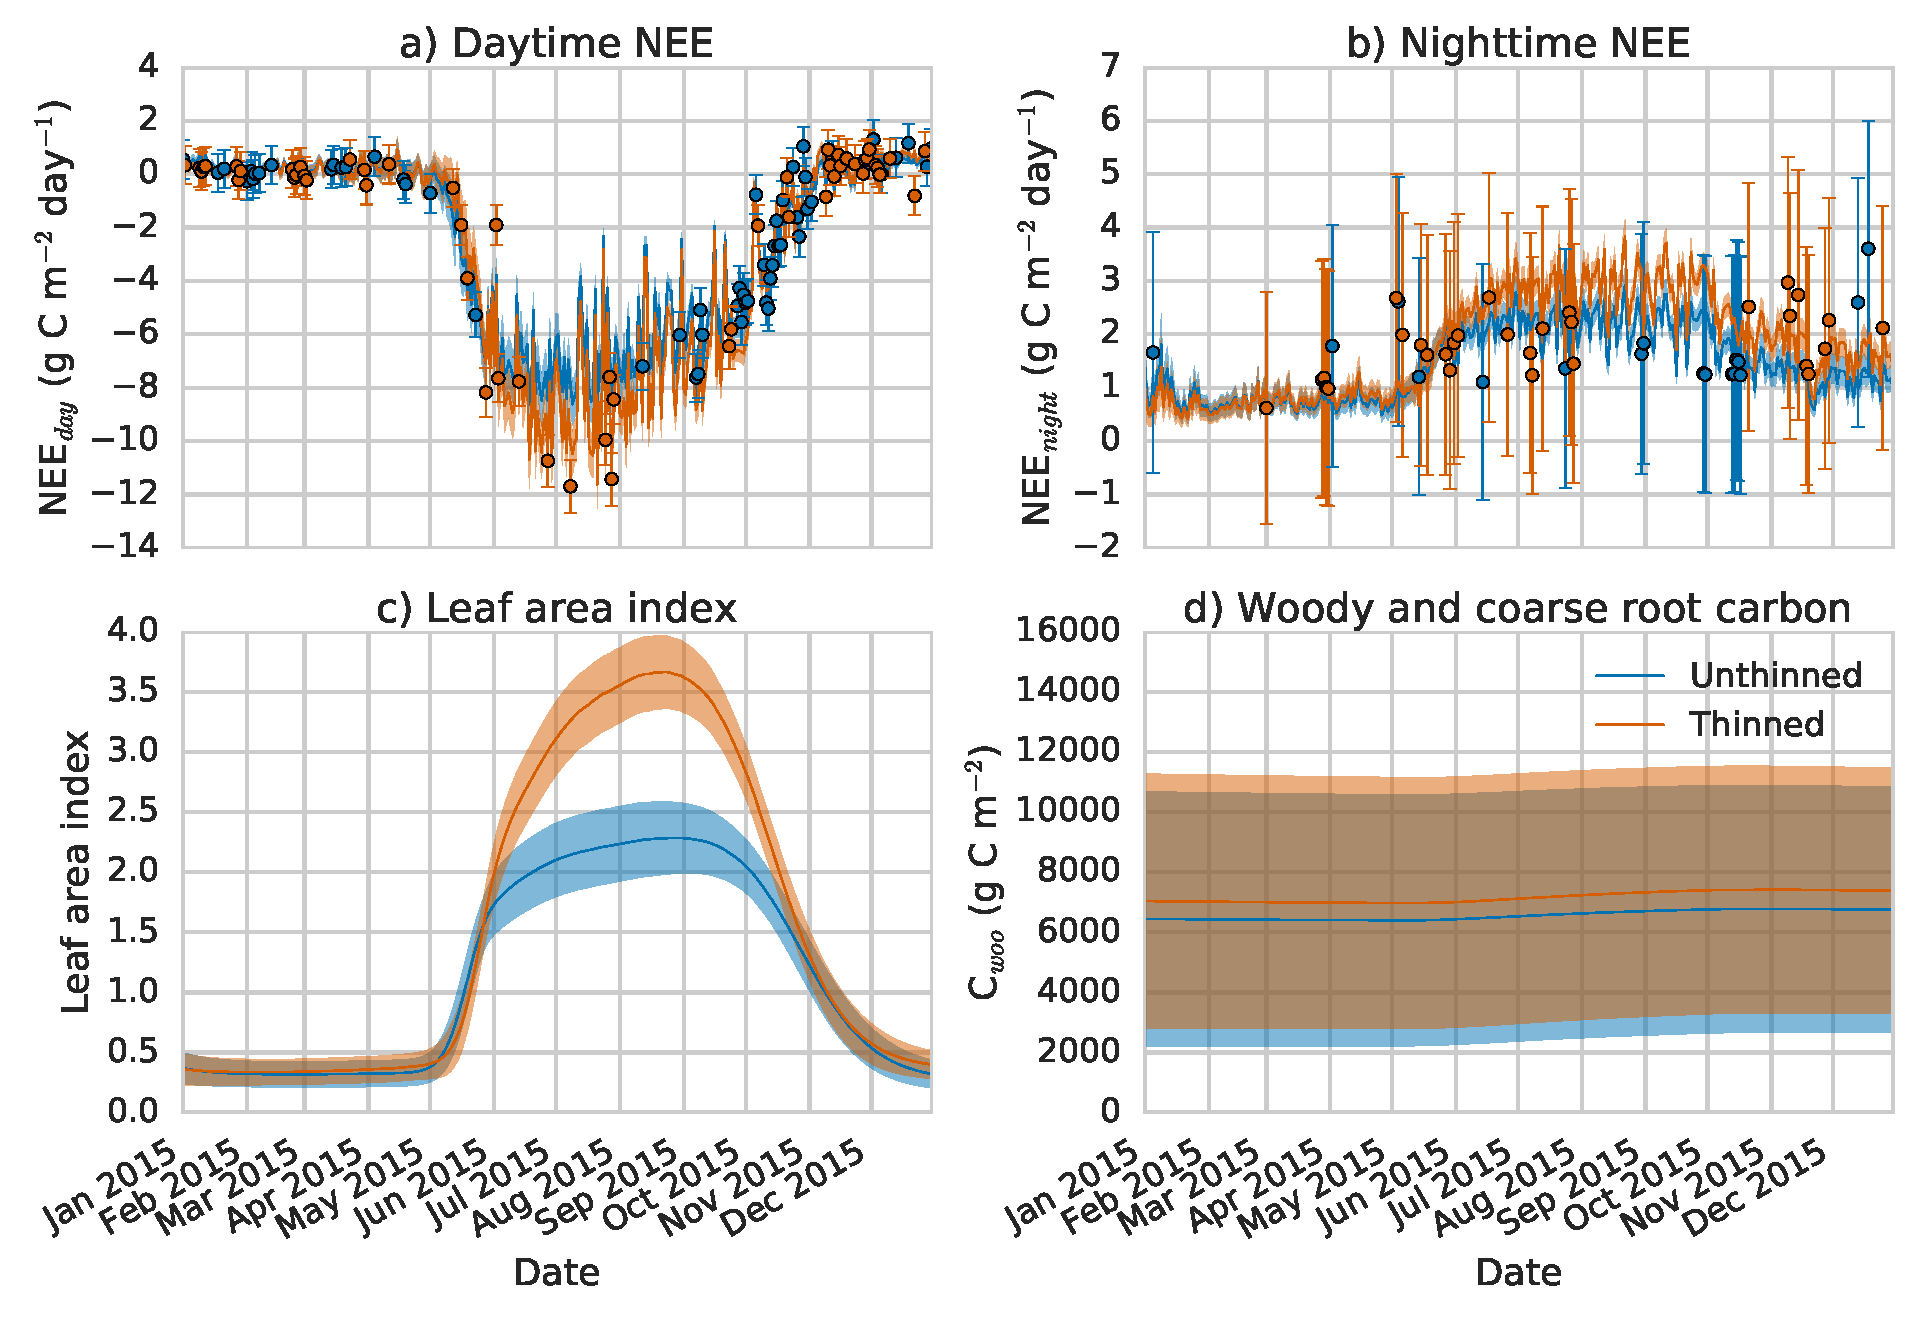
\includegraphics[width=\textwidth]{obs_compa.pdf}
\caption{Experiment A: 2015 unthinned and thinned forest observations and model trajectories after assimilation. Blue line: model trajectory after assimilation of unthinned data, blue shading: uncertainty in model trajectory after assimilation (\(\pm\) 1 standard deviation), blue dots: unthinned observations with error bars, orange line: model trajectory after assimilation of thinned data, orange shading: uncertainty in model trajectory after assimilation (\(\pm\) 1 standard deviation), orange dots: thinned observations with error bars.}
 \label{fig:obscompa}
 \end{figure}
 
 \begin{figure}[ht]
    \centering
        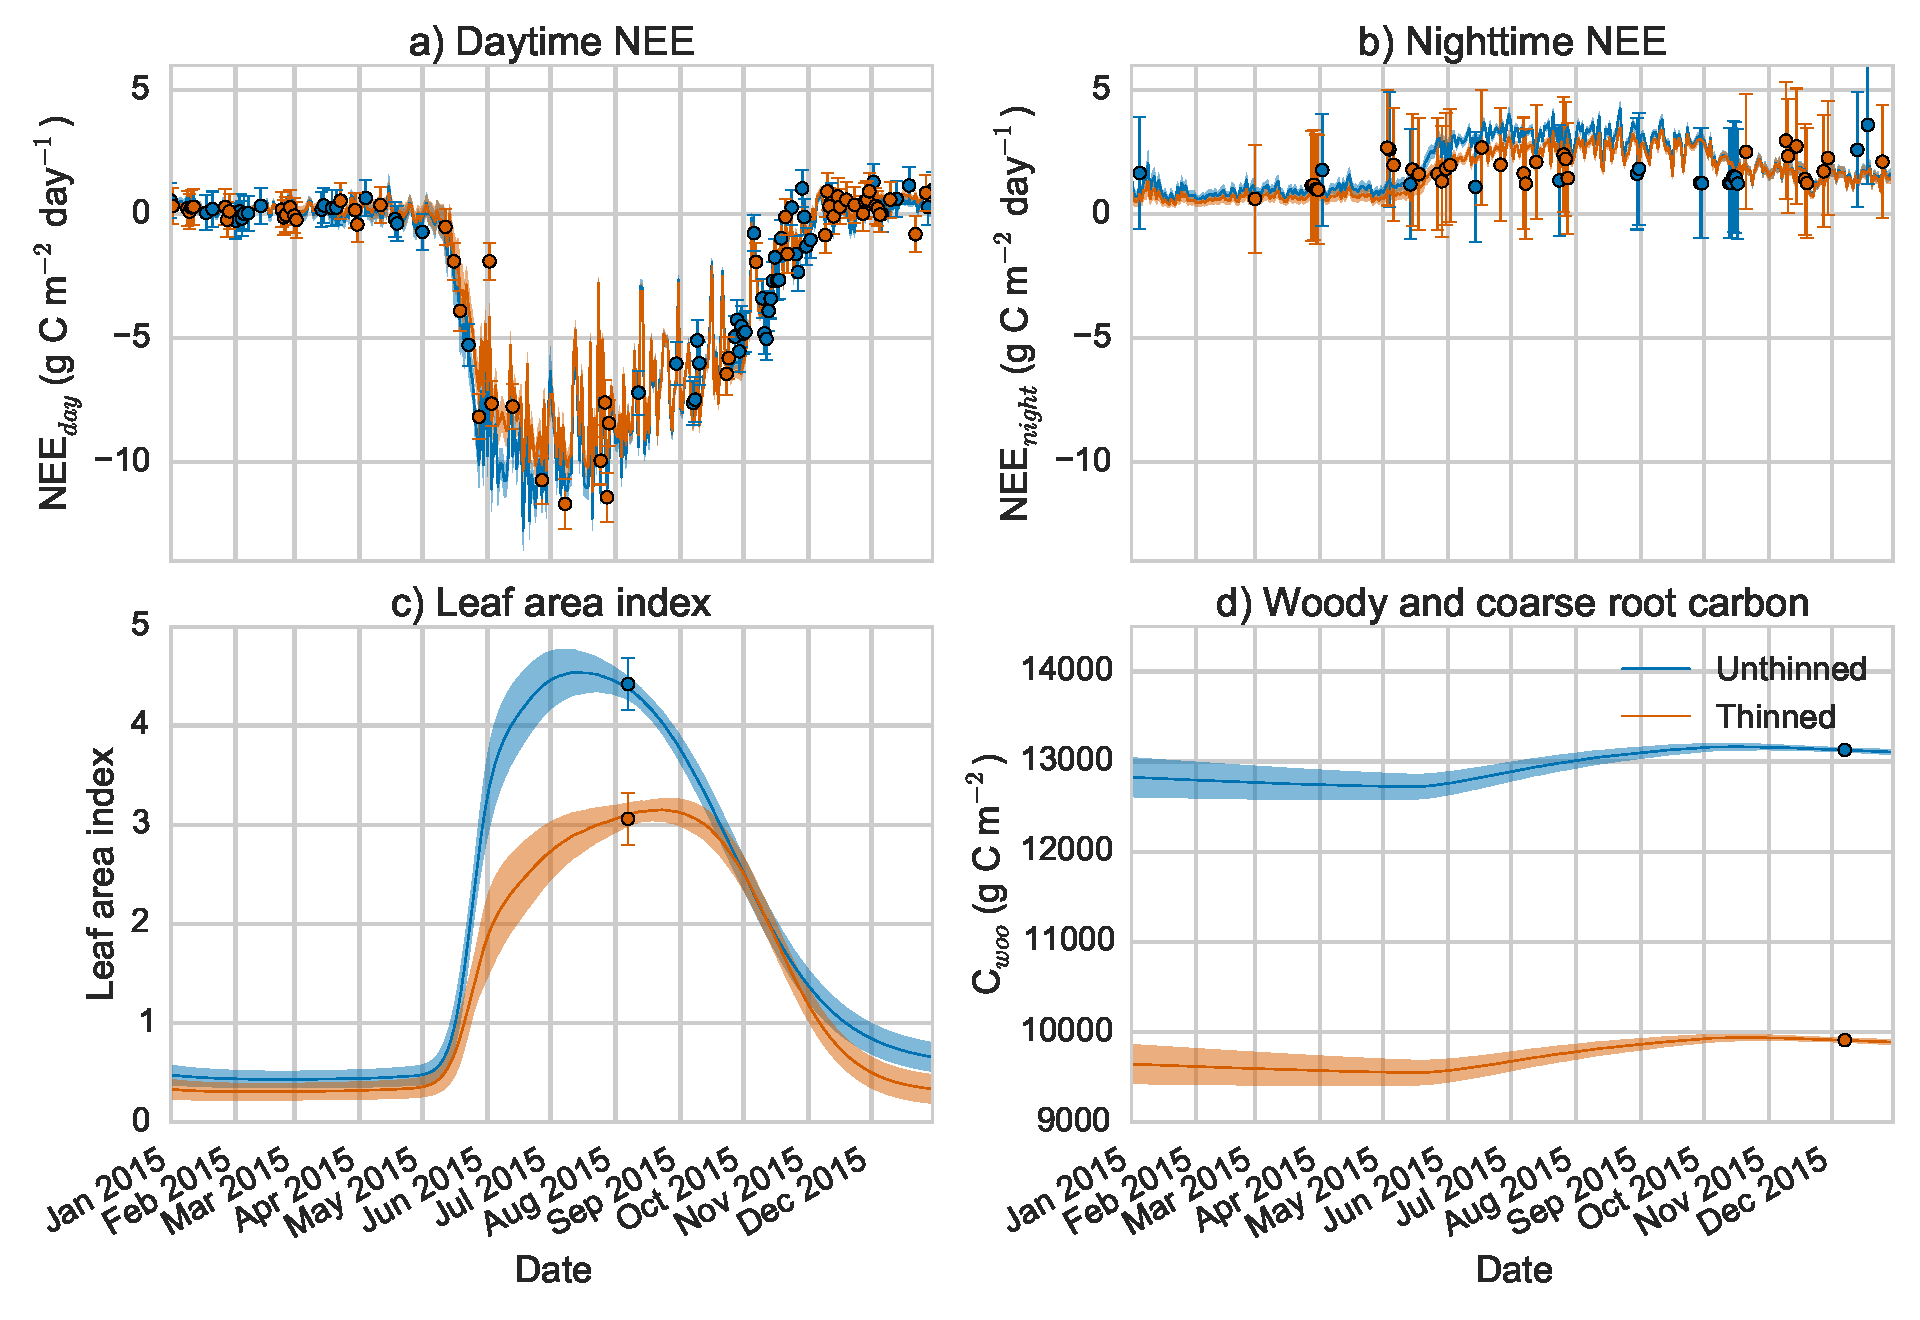
\includegraphics[width=\textwidth]{obs_compc.pdf}
\caption{Experiment C: 2015 unthinned and thinned forest observations and model trajectories after assimilation. Colour, lines and dots have the same meaning as described in Figure~\ref{fig:obscompa}. Figure c) and d) now also include observations of LAI and \(C_{woo}\) (dots).}
 \label{fig:obscompc}
 \end{figure}

\begin{table}[ht] 
	\caption{Root-mean-square error of model fit to observations for the prior model and all experiments after data assimilation.}
\begin{center}
	\begin{tabular}{| l | l | l | l | l | l}
	\hline
	\multicolumn{5}{| c |}{Unthinned forest} \\ \hline
	Exp. & NEE\(_{day}\) & NEE\(_{night}\)  & LAI & \(C_{woo}\)  \\ \hline
	Prior & 1.25 \(\text{g C m}^{-2}~\text{day}^{-1}\) & 1.02 \(\text{g C m}^{-2}~\text{day}^{-1}\)  & 0.43 & 5507 \(\text{g C m}^{-2}\)  \\ \hline
	A & 0.61 \(\text{g C m}^{-2}~\text{day}^{-1}\) & 0.83 \(\text{g C m}^{-2}~\text{day}^{-1}\)  & 2.16 & 6361 \(\text{g C m}^{-2}\)  \\ \hline
	B & 0.75 \(\text{g C m}^{-2}~\text{day}^{-1}\) & 0.93 \(\text{g C m}^{-2}~\text{day}^{-1}\) & 0.04 & 5987 \(\text{g C m}^{-2}\)  \\ \hline
	C & 0.75 \(\text{g C m}^{-2}~\text{day}^{-1}\) & 0.93 \(\text{g C m}^{-2}~\text{day}^{-1}\) & 0.04 & 0.16 \(\text{g C m}^{-2}\)  \\ \hline
	\multicolumn{5}{| c |}{Thinned forest} \\ \hline
	Exp. & NEE\(_{day}\) & NEE\(_{night}\)  & LAI & \(C_{woo}\)  \\ \hline
	Prior & 1.05 \(\text{g C m}^{-2}~\text{day}^{-1}\) & 0.61 \(\text{g C m}^{-2}~\text{day}^{-1}\) & 1.79 & 2285 \(\text{g C m}^{-2}\)  \\ \hline
	A & 0.63 \(\text{g C m}^{-2}~\text{day}^{-1}\) & 0.54 \(\text{g C m}^{-2}~\text{day}^{-1}\) & 0.55 & 2505 \(\text{g C m}^{-2}\)  \\ \hline
	B & 0.63 \(\text{g C m}^{-2}~\text{day}^{-1}\) & 0.56 \(\text{g C m}^{-2}~\text{day}^{-1}\) & 0.04 & 2241 \(\text{g C m}^{-2}\)  \\ \hline
	C & 0.63 \(\text{g C m}^{-2}~\text{day}^{-1}\) & 0.56 \(\text{g C m}^{-2}~\text{day}^{-1}\) & 0.04 & 0.07 \(\text{g C m}^{-2}\)  \\ \hline
	\end{tabular}
	\label{table:mod_rmse}
\end{center} 
\end{table}

Table~\ref{table:fluxes} shows the cumulative annual fluxes for the year 2015 for the three experiments. In all three experiments there is no significant difference between the net carbon uptake for the thinned and unthinned forest. We can see that both experiments B and C predict very similar cumulative fluxes, suggesting that the assimilated observations of \(C_{woo}\) have not had much impact on the model carbon dynamics for this time period. Because the rate parameters controlling this pool are relatively slow it is likely that observations of \(C_{woo}\) will become much more important over longer time-scales. Here we have only assimilated a single observation of \(C_{woo}\) for either side of the forest; if multiple observations of \(C_{woo}\) were available throughout time this would give us an estimate of the rate of woody biomass accumulation, providing an important constraint on the carbon assimilation of the forest. Experiments A and C both predict no significant difference in the net ecosystem carbon uptake between the thinned and unthinned forest. However, the partitioning of this carbon uptake between GPP and total ecosystem respiration (TER) is significantly different, with experiment A predicting increased TER and GPP after thinning and experiment C predicting reduced TER and GPP after thinning. This can be seen more clearly in Figure~\ref{fig:cum_flux}. The difference between the results of experiment A and C highlights the issue that NEE is the difference between two large fluxes (NEE = -GPP + TER) and we can therefore find an accurate prediction of NEE despite under/overestimating both GPP and TER. Therefore, care should be taken when interpreting model results based solely on NEE data, especially in this case, as we have seen that the partitioning of the NEE data between the thinned and unthinned forest has introduced a bias into our dataset. If we were to base our analysis on experiment A we would assume that the thinning had caused an increase in ecosystem respiration and that this had been compensated for by an increase in GPP. This is the opposite conclusion to the one we find in experiment C when we include observations relating to the structure of the forest. 

\begin{table}[ht] 
	\caption{Total annual fluxes and standard deviations for 2015 after assimilation \((\text{g C m}^{-2})\).}
\begin{center}
	\begin{tabular}{| l | l | l | l | l}
	\hline
	\multicolumn{4}{| c |}{Unthinned forest} \\ \hline
	Flux & Experiment A & Experiment B & Experiment C \\ \hline
	NEE & \(-379\pm 99\) & \(-425\pm113\) & \(-426\pm116\) \\ \hline
	GPP & \(1648\pm 159\) & \(2191\pm 87\) & \(2193\pm83\) \\ \hline
	TER & \(1267\pm 150\) & \(1766\pm146\) & \(1767\pm146\) \\ \hline
	\multicolumn{4}{| c |}{Thinned forest} \\ \hline
	Flux & Experiment A & Experiment B & Experiment C \\ \hline
	NEE & \(-394\pm 81\) & \(-421\pm73\) & \(-420\pm78\) \\ \hline
	GPP & \(1976\pm 112\) & \(1855\pm75\) & \(1856\pm80\) \\ \hline
	TER & \(1582\pm 134\) & \(1435\pm100\) & \(1436\pm109\) \\ \hline
	\end{tabular}
	\label{table:fluxes}
\end{center} 
\end{table}

\begin{figure}[ht]
    \centering
        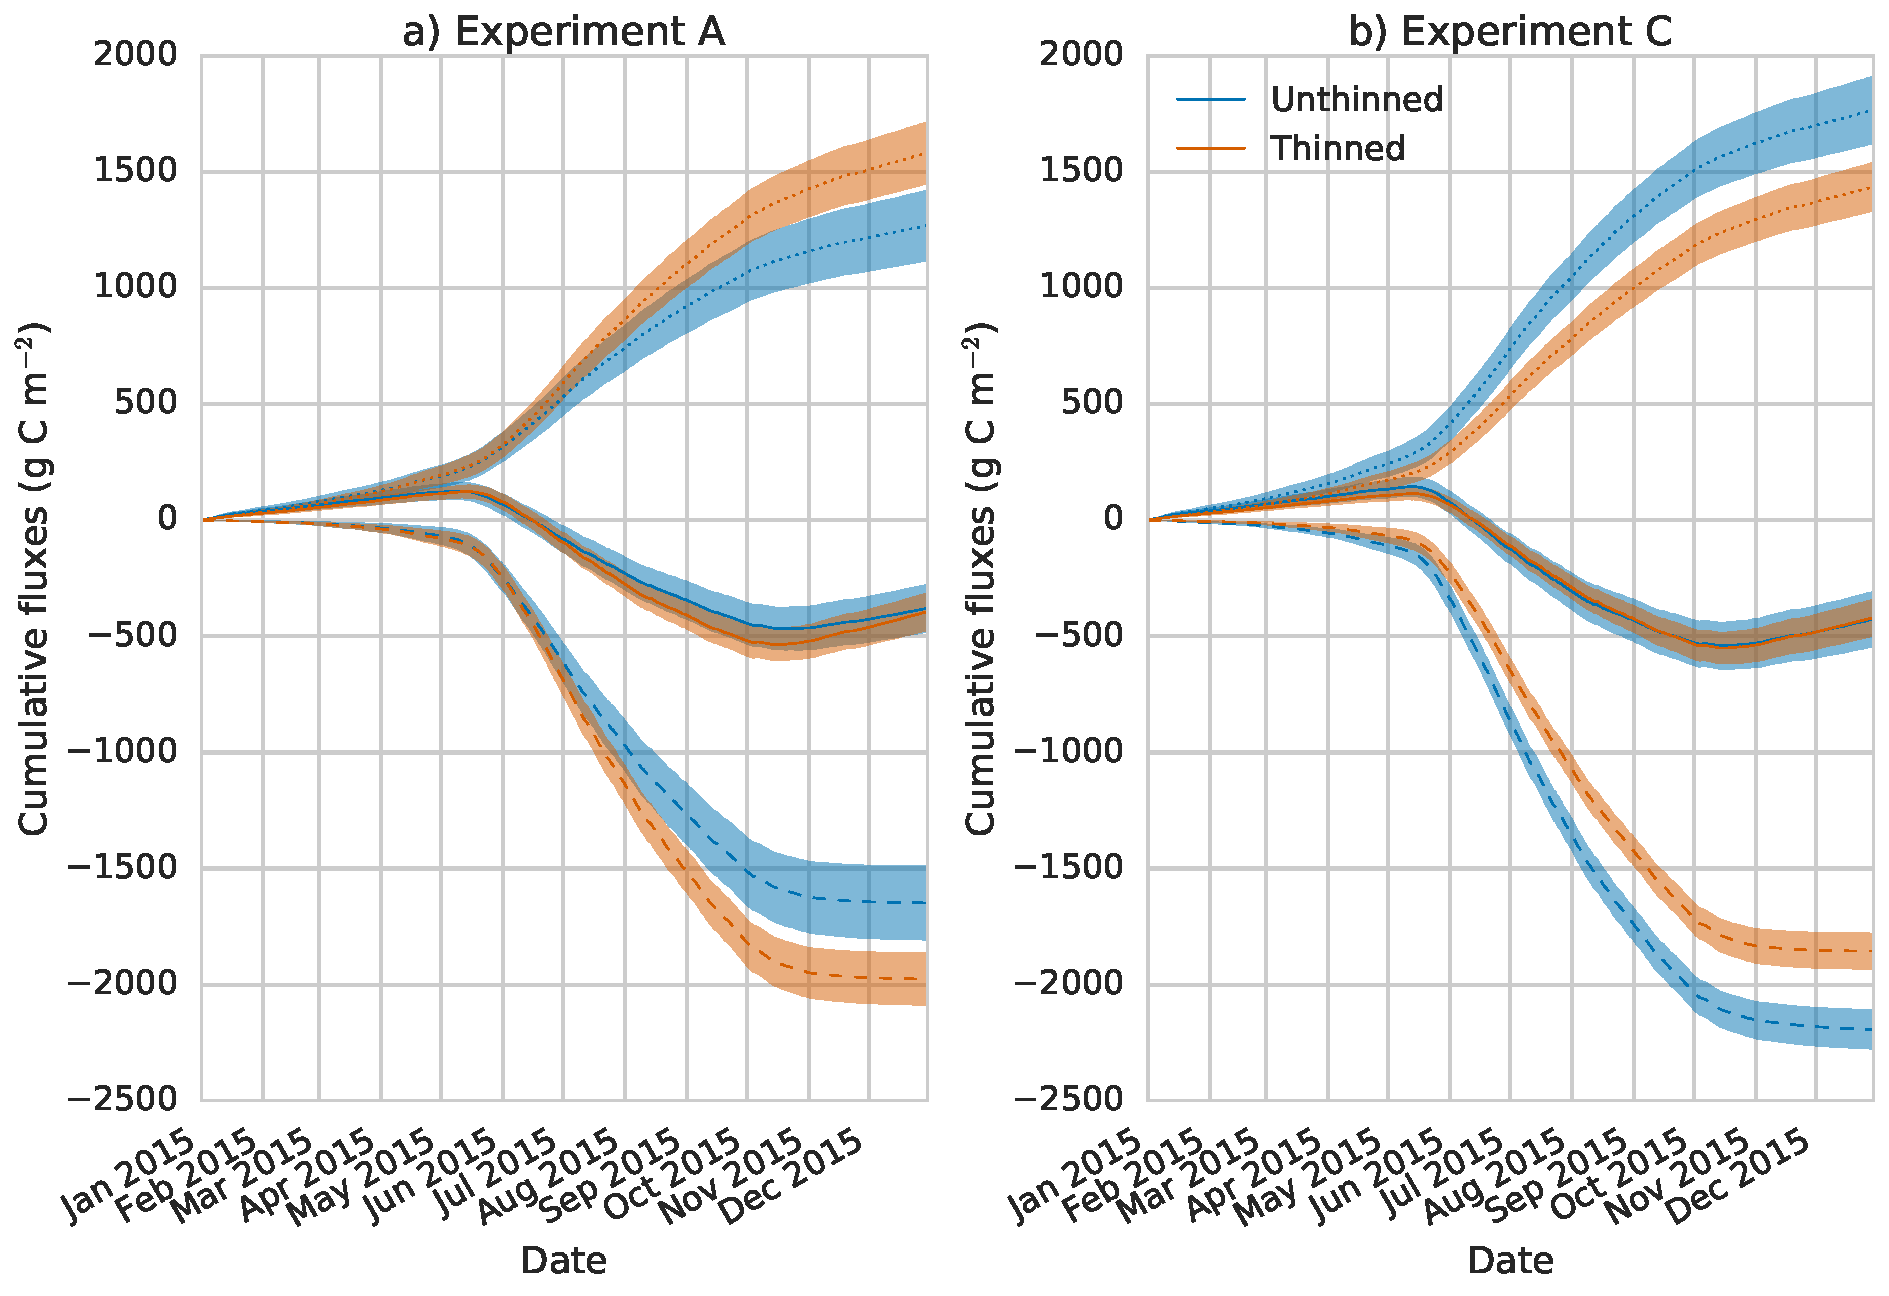
\includegraphics[width=\textwidth]{flux_part.pdf}
    \caption{Experiment A \& C: 2015 unthinned and thinned forest model trajectories for cumulative fluxes after assimilation. Solid line: cumulative NEE, dotted line: cumulative ecosystem respiration, dashed line: cumulative GPP. Colour and shading has the same meaning as in Figure~\ref{fig:obscompa}.} \label{fig:cum_flux}
\end{figure}


\begin{figure}[ht]
    \centering
        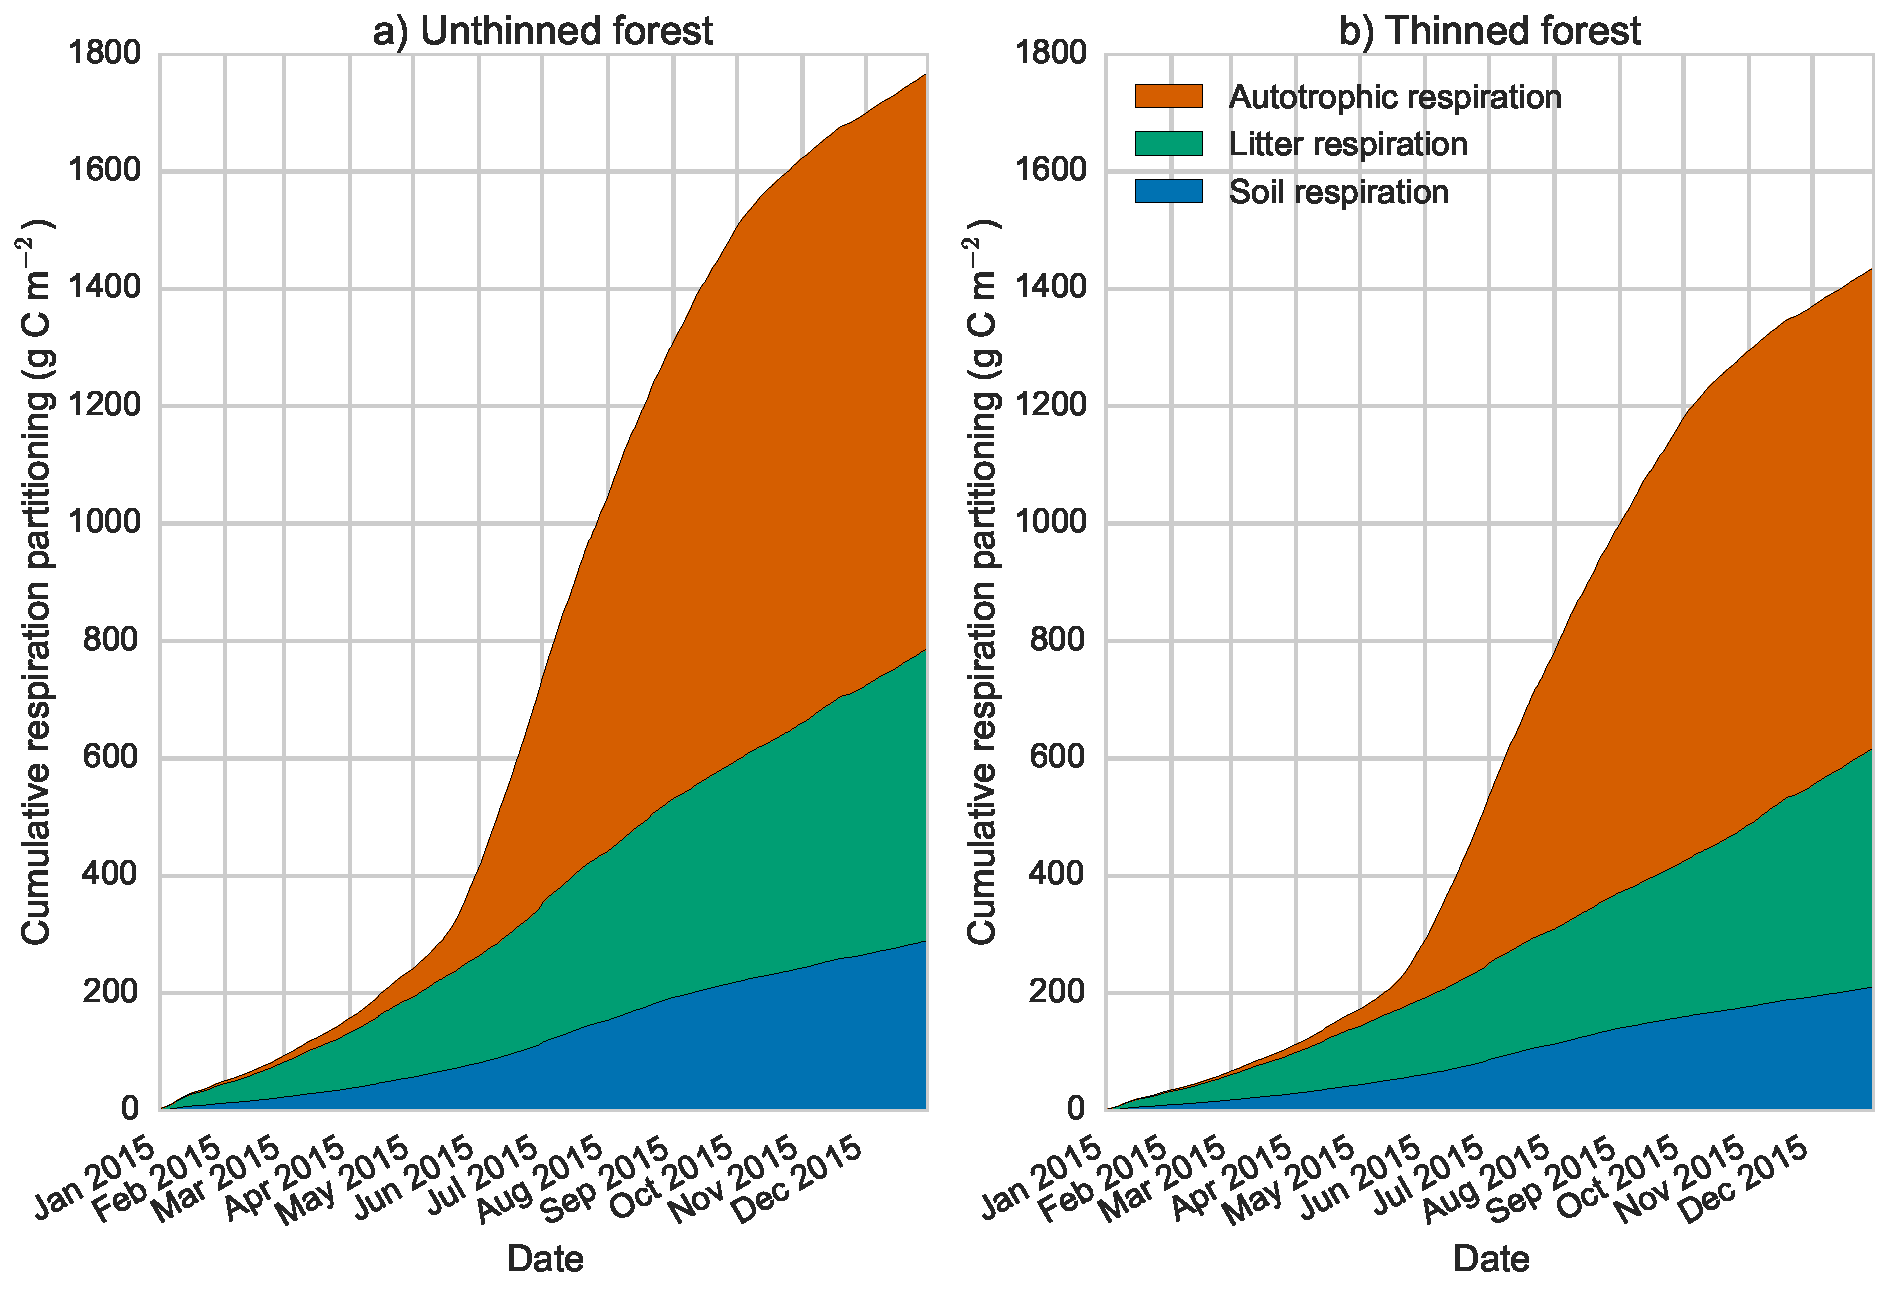
\includegraphics[width=\textwidth]{resp_partc.pdf}
    \caption{Experiment C: 2015 unthinned and thinned forest model trajectory for cumulative total ecosystem respiration after assimilation and its partitioning between total autotrophic respiration and heterotrophic respiration from litter and soil.} \label{fig:rt_part}
\end{figure}

In Figure~\ref{fig:rt_part} we show the partitioning of cumulative ecosystem respiration for the year 2015 between total autotrophic respiration and heterotrophic respiration from litter and soil for both the unthinned and thinned forest in experiment C. Here we can see the strong dependance of autotrophic respiration on GPP with the growth rate being much greater between June 2015 - September 2015 (when GPP will be of greater magnitude). For heterotrophic respiration the growth rate is more constant throughout the whole year. Total ecosystem respiration is reduced by 331\(~\text{g C m}^{-2}\) for the thinned forest when compared to the unthinned forest, with reductions in both heterotrophic and autotrophic respiration of 169\(~\text{g C m}^{-2}\) and 162\(~\text{g C m}^{-2}\) respectively.    

\begin{figure}[ht]
    \centering
    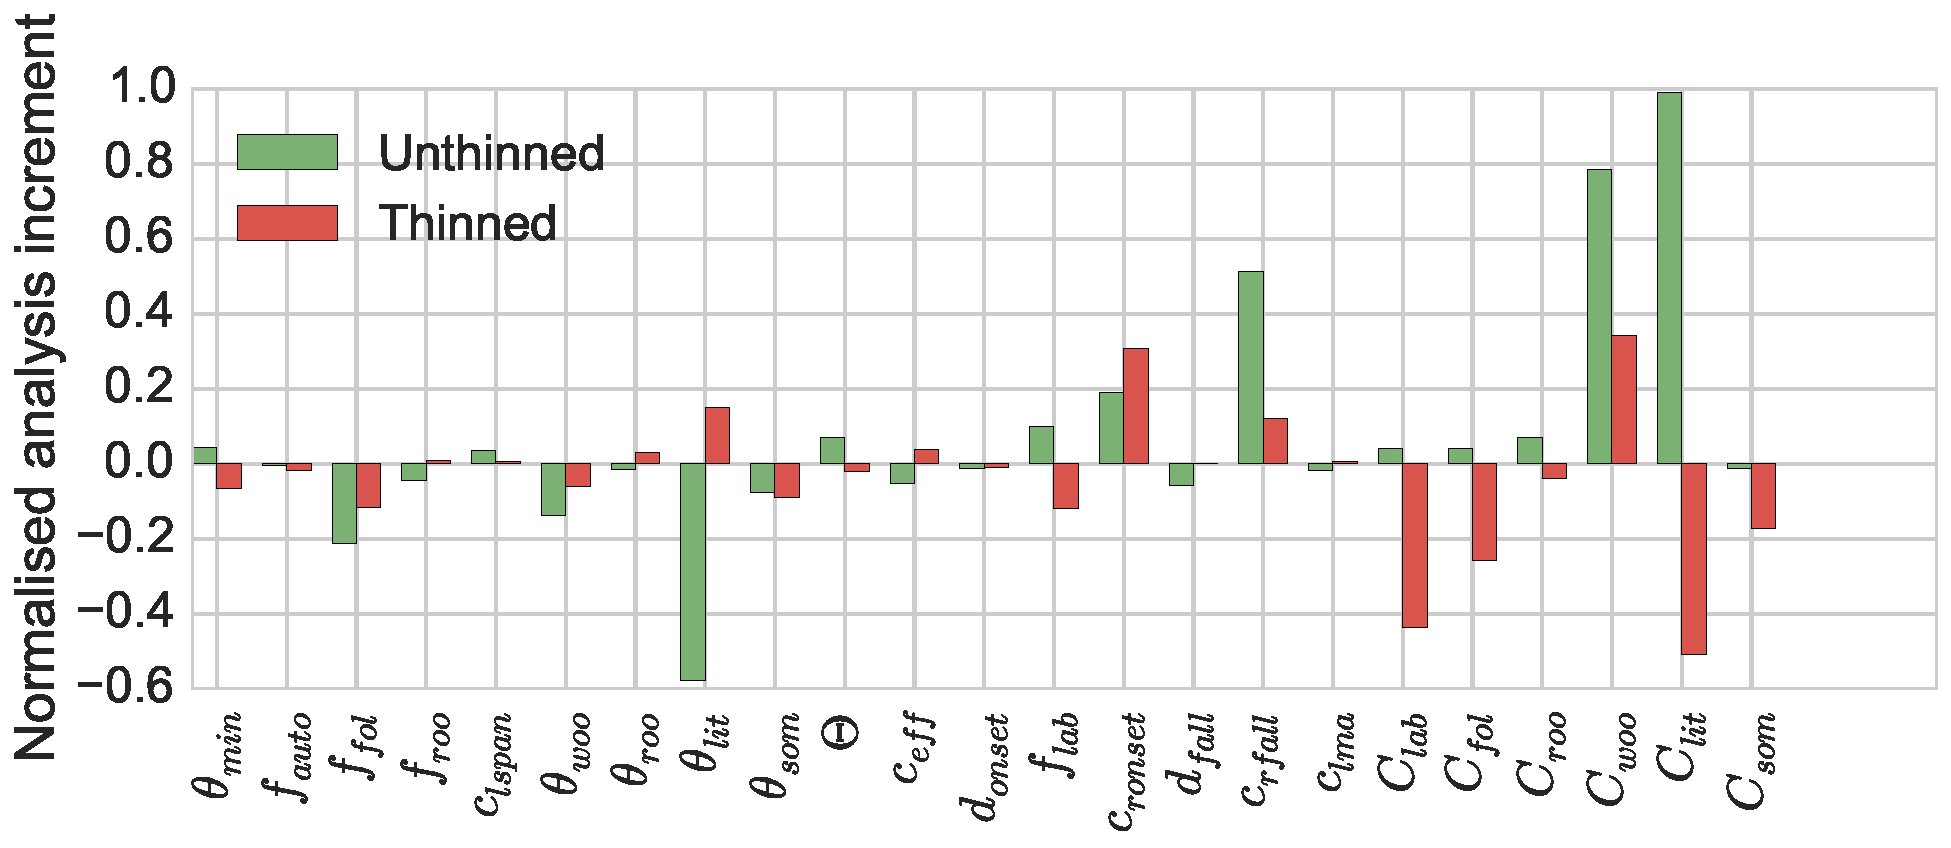
\includegraphics[width=0.8\textwidth]{xa_incc.pdf}
    \caption{Experiment C: normalised change in parameter and state variables after data assimilation \big($\frac{(\textbf{x}^a(j) - \textbf{x}^b(j))}{\textbf{x}^b(j)}$\big) for the unthinned and thinned forest. Explanation of parameter and state variable symbols in table~\ref{table:xbvars}.}
    \label{fig:xa_inc}
\end{figure}

Figure~\ref{fig:xa_inc} shows the change in parameter and initial state values for the thinned and unthinned forest after assimilating all observations in experiment C. It is important to note that this is the difference when compared to our prior model estimate, which was found by assimilating only eddy covariance, LAI and leaf mass per area observations from 2012 and 2013. We therefore expect changes in parameter and state values for both the thinned and unthinned forest, as we are assimilating new data streams. This is particularly noticeable in the carbon pool state variables in Figure~\ref{fig:xa_inc}. Constraints on the carbon pool state variables are provided by the assimilated observations of woody biomass and coarse roots (\(C_{woo}\)), LAI and leaf mass per area (\(c_{lma}\)). LAI and \(c_{lma}\) give us a constraint on foliar carbon (\(C_{fol}\)) as LAI \(= \frac{C_{fol}}{c_{lma}} \). We can see the values for the model predicted carbon pools are as we might expect with the thinned forest having less carbon in all pools when compared to the unthinned forest. For litter carbon (\(C_{lit}\)) we expect a reduction in input of leaf litter for the thinned forest and, although there might be increased woody debris after thinning, this is much less readily decomposed and so possibly has little impact in the year after thinning \citep{wilkinson2016}. The difference in predicted soil carbon content (\(C_{som}\)) between the thinned and unthinned forest is consistent with studies analysing soil carbon contents after felling \citep{Hernesmaa2005777}. For the parameters the biggest changes appear to be in the litter carbon turnover rate parameter (\(\theta_{lit}\)), with the retrieved parameter being significantly reduced for the unthinned forest when compared to the thinned. However, we still see reduced total litter respiration in Figure~\ref{fig:rt_part} for the thinned forest compared to the unthinned forest. This is due to the significant difference in litter carbon content (\(C_{lit}\)) for both sides, with the unthinned forest having a much higher litter carbon content than the thinned forest. The large change in the \(\theta_{lit}\) parameter between the two sides is therefore compensating for an overestimated difference in litter carbon content between the two sides.    
 \clearpage
 
 
\section{Discussion}
{\color{blue}In this paper we have investigated the possible explanations for the observation that a thinning event, where approximately $46\%$ of trees were removed from the study site, had no impact on net ecosystem carbon uptake. We used data assimilation to combine observations and prior model predictions of ecosystem carbon balance in order to understand how the state of an ecosystem might be altered after a disturbance event.} We conducted three experiments assimilating different combinations of available data streams. For all experiments we find no significant change in net carbon uptake for the studied ecosystem following stand thinning. This is consistent with other studies of ecosystem carbon dynamics following thinning {\color{blue}\citep{vesala2005effect, moreaux2011paired, dore2012recovery, wilkinson2016}}. We find different reasons for this unchanged carbon uptake dependent on which data streams are assimilated. When only assimilating NEE observations we find increased ecosystem respiration and increased GPP post-disturbance. These results are unreliable due to bias introduced into the NEE dataset from partitioning between the thinned and unthinned forest. From our most confident estimate, where all available observations are assimilated, the model shows that reductions in GPP, following a decrease in total leaf area post-thinning, are being offset by simultaneous reductions in ecosystem respiration. This is in contrast to current suggestions that reduced canopy photosynthesis is compensated for by increased GPP by ground vegetation post-thinning \citep{vesala2005effect, moreaux2011paired, dore2012recovery, wilkinson2016}.

%however does support work investigating the effect of insect disturbance \citep{ELE:ELE12097}.

Our results show a decrease in both autotrophic and heterotrophic respirations following thinning. We follow the definition of \citet{heinemeyer2012exploring} and characterise below ground autotrophic respiration as respiration from roots, mycorrhizal fungi and other micro-organisms dependent on the priming of soils with labile carbon compounds from roots. Heterotrophic respiration is respiration by microbes not directly dependent on autotrophic substrate; however, the largest fraction of heterotrophic respiration is based on the decomposition of young organic matter (e.g. leaves and fine roots) whose availability also depends on the GPP of an ecosystem \citep{GCB:GCB412}. We find similar decreases in both heterotrophic and autotrophic respiration for the thinned forest when compared with the unthinned forest. While it has been shown that heterotrophic respiration can decrease after disturbance events \citep{PCE:PCE1053}, it is possible we overestimate the reduction in heterotrophic respiration and underestimate the reduction in autotrophic respiration. This is understandable as we have assimilated no data on this partitioning. Also our model description of autotrophic respiration is simple (described as a constant fraction of GPP) and therefore the heterotrophic respiration component of the model might compensate and in this instance describe the behaviour of mycorrhizal fungi and other microbes commonly categorised in the autotrophic component of respiration.   

In a study measuring soil CO\(_{2}\) fluxes over 4 years at the Straits Inclosure (the study site in this paper) \citet{heinemeyer2012exploring} showed a large 56\% contribution of autotrophic respiration (characterised as root and mycorrhizal respiration) to total measured soil respiration. \citet{heinemeyer2012exploring} also suggested that mycorrhizal fungi play a role in priming the turnover of soil organic carbon by other microbes, with evidence from \citet{talbot2008decomposers}. \citet{hogberg2006towards} find similar figures for the autotrophic contribution to total soil respiration, with around half or more of all soil respiration being driven by recent photosynthesis. \citet{heinemeyer2012exploring} discuss the possibility of this tight coupling between GPP and ecosystem respiration leading to an upper limit for forest CO\(_{2}\) uptake due to increased GPP leading to increased respiration, which is also discussed by \citet{heath2005rising}. Our results support this hypothesis, as ecosystem respiration scales with GPP after approximately 46\% of trees are removed from the study site, meaning that we find no significant change in net ecosystem carbon uptake after thinning.   

Studies analysing eddy covariance flux records also find no significant change in the net ecosystem exchange of CO\(_{2}\) after thinning \citep{vesala2005effect, moreaux2011paired, dore2012recovery, wilkinson2016}. {\color{blue}(4) \citet{vesala2005effect} used a model of light interception and ground vegetation photosynthesis to show that the unchanged NEE was due to increased GPP by ground vegetation (following increased light availability and reduced competition) compensating for increases in heterotrophic respiration and reduced canopy photosynthesis post-thinning. Similar conclusions are drawn in \citet{moreaux2011paired} by destructively sampling ground vegetation and showing an increase in biomass post-thinning}. We do not find evidence to support such conclusions and instead suggest that reduced ecosystem respiration is the most important component for the unchanged NEE of the forest following thinning. However, it is important to note that our measurements of LAI are made at approximately 1~m above the forest floor, which means that our measurements of LAI do not account for ground vegetation. Therefore, any effect of this ground vegetation is not simulated by our model. Despite this, observations made during multiple walks of the three established transects find no evidence of increased ground vegetation in the year after thinning. In fact much of the ground vegetation and subcanopy was removed during thinning and did not appear to have recovered in the following year. At longer time-scales re-growth of the subcanopy and ground vegetation will play an important role in increased productivity. Our results suggest that this increased productivity would also be met with subsequent increases in ecosystem respiration.

{\color{blue}Data assimilation provides a valuable alternative to more common statistical analyses of flux data records to calculate constituent ecosystem carbon fluxes, as it allows for the combination of many distinct data streams and the dynamics of a physically meaningful model to construct our solution. We have shown that basing our results on a single data stream (NEE) can give us much different conclusions than when all data streams are assimilated. In this work we have been strict on the quality control procedures for NEE data, and have allowed no gap filling, to ensure we base our results on only the best quality true observations. This and the partitioning of the NEE data set between the thinned and unthinned areas of forest has resulted in a distinct data gap during the growing season for the thinned site NEE, as discussed in section~\ref{sec:results}. From the data assimilation experiments conducted we have shown that the combination of multiple distinct data steams has helped to reduce the impact of this data gap on assimilation results. }  

The effect of disturbance is poorly characterised in current land surface and global climate models \citep{running2008ecosystem}; it is important to better understand how parameters and carbon pools might change following disturbance. DALEC2 and many other ecosystem models assume that respiration rates are proportional to carbon pool size. It has been suggested that although this assumption works well in equilibrium conditions it may not allow such models to predict ecosystem carbon dynamics following disturbance \citep{schimel2003implications}. The data assimilation techniques in this paper present a way for these simple models to cope with step changes in ecosystem behaviour, by allowing parameters and carbon pools to be updated following disturbance events. 


%From the assimilation of multiple data streams with a model of ecosystem carbon balance we find evidence that reduced heterotrophic respiration following disturbance allows a managed woodland to exhibit an unchanged net carbon uptake when compared against an undisturbed section of the same woodland. 

\section{Conclusion}

In this work we have presented novel methods for understanding ecosystem responses to disturbance by using data assimilation. Assimilating all available data streams after an event of disturbance with a prior model prediction allows us to assess changes to model parameter and state variables due to this disturbance. We have also created modified observation operators to allow for the assimilation of daytime and nighttime NEE observations with a daily time-step model. This negated the need for model modification and increased the number of observations by a factor of 4.25.

Our {\color{blue}modeled} estimates show no significant change in net ecosystem carbon uptake after a thinning event in 2014 where approximately 46\% of trees were removed from the studied area. Similar results were also found following a thinning activity in 2007 \citep{wilkinson2016}. From our optimised model we find that reduced ecosystem respiration is the main reason for this unchanged net ecosystem carbon uptake. Therefore, even for a decrease in GPP following thinning, there is no significant change in NEE. We hypothesise this reduction in ecosystem respiration is due to reduced input of autotrophic substrate following thinning, meaning both autotrophic and heterotrophic respiration are reduced. These results support work suggesting that GPP is the dominant driver for ecosystem respiration  \citep{GCB:GCB412, PCE:PCE1053, hogberg2006towards, heinemeyer2012exploring, ELE:ELE12097}. This has implications for future predictions of land surface carbon uptake and whether forests will continue to sequester atmospheric CO\(_{2}\) at similar rates, or if they will be limited by increased GPP leading to increased respiration. 



%Text here ===>>>

%%

%  Numbered lines in equations:
%  To add line numbers to lines in equations,
%  \begin{linenomath*}
%  \begin{equation}
%  \end{equation}
%  \end{linenomath*}



%% Enter Figures and Tables near as possible to where they are first mentioned:
%
% DO NOT USE \psfrag or \subfigure commands.
%
% Figure captions go below the figure.
% Table titles go above tables;  other caption information
%  should be placed in last line of the table, using
% \multicolumn2l{$^a$ This is a table note.}
%
%----------------
% EXAMPLE FIGURE
%
% \begin{figure}[h]
% \centering
% when using pdflatex, use pdf file:
% \includegraphics[width=20pc]{figsamp.pdf}
%
% when using dvips, use .eps file:
% \includegraphics[width=20pc]{figsamp.eps}
%
% \caption{Short caption}
% \label{figone}
%  \end{figure}
%
% ---------------
% EXAMPLE TABLE
%
% \begin{table}
% \caption{Time of the Transition Between Phase 1 and Phase 2$^{a}$}
% \centering
% \begin{tabular}{l c}
% \hline
%  Run  & Time (min)  \\
% \hline
%   $l1$  & 260   \\
%   $l2$  & 300   \\
%   $l3$  & 340   \\
%   $h1$  & 270   \\
%   $h2$  & 250   \\
%   $h3$  & 380   \\
%   $r1$  & 370   \\
%   $r2$  & 390   \\
% \hline
% \multicolumn{2}{l}{$^{a}$Footnote text here.}
% \end{tabular}
% \end{table}

%% SIDEWAYS FIGURE and TABLE 
% AGU prefers the use of {sidewaystable} over {landscapetable} as it causes fewer problems.
%
% \begin{sidewaysfigure}
% \includegraphics[width=20pc]{figsamp}
% \caption{caption here}
% \label{newfig}
% \end{sidewaysfigure}
% 
%  \begin{sidewaystable}
%  \caption{Caption here}
% \label{tab:signif_gap_clos}
%  \begin{tabular}{ccc}
% one&two&three\\
% four&five&six
%  \end{tabular}
%  \end{sidewaystable}

%% If using numbered lines, please surround equations with \begin{linenomath*}...\end{linenomath*}
%\begin{linenomath*}
%\begin{equation}
%y|{f} \sim g(m, \sigma),
%\end{equation}
%\end{linenomath*}

%%% End of body of article

%%%%%%%%%%%%%%%%%%%%%%%%%%%%%%%%
%% Optional Appendix goes here
%
% The \appendix command resets counters and redefines section heads
%
% After typing \appendix
%
%\section{Here Is Appendix Title}
% will show
% A: Here Is Appendix Title
%
%\appendix
%\section{Here is a sample appendix}
\appendix
\section{Appendix} \label{sec:appendix}

\subsection{DALEC2 equations} \label{sec:dalec_eqns}

The model equations for the carbon pools at day $i$ are as follows:

\begin{align}
GPP^{i} &= ACM(C_{fol}^{i-1}, c_{lma}, c_{eff}, \Psi) \label{GPP}
\\C_{lab}^{i}&=C_{lab}^{i-1}+(1-f_{auto})(1-f_{fol})f_{lab}GPP^{i}-\Phi _{on}C_{lab}^{i-1}, \label{daleclab}
\\C_{fol}^{i}&=C_{fol}^{i-1}+\Phi_{on}C_{lab}^{i-1}+(1-f_{auto})f_{fol}GPP^{i}-\Phi_{off}C_{fol}^{i-1}, \label{dalec1}
\\C_{roo}^{i}&=C_{roo}^{i-1}+(1-f_{auto})(1-f_{fol})(1-f_{lab})f_{roo}GPP^{i}-\theta_{roo}C_{roo}^{i-1}, 
\\C_{woo}^{i}&=C_{woo}^{i-1}+(1-f_{auto})(1-f_{fol})(1-f_{lab})(1-f_{roo})GPP^{i}-\theta_{woo}C_{woo}^{i-1}, 
\\C_{lit}^{i}&=C_{lit}^{i-1}+\theta_{roo}C_{roo}^{i-1}+\Phi_{off}C_{fol}^{i-1}-(\theta_{lit}+\theta_{min})e^{\Theta T^{i-1}}C_{lit}^{i-1}, 
\\C_{som}^{i}&=C_{som}^{i-1}+\theta_{woo}C_{woo}^{i-1}+\theta_{min}e^{\Theta T^{i-1}}C_{lit}^{i-1}-\theta_{som}e^{\Theta T^{i-1}}C_{som}^{i-1}, \label{dalec5}
\end{align}
where $T^{i-1}$ is the daily mean temperature, $\Psi$ represents the meteorological driving data used in the $GPP$ function and $\Phi_{on} / \Phi_{off}$ are functions controlling leaf-on and leaf-off. Descriptions for each model parameter used in equations \eqref{GPP} to \eqref{dalec5} are included in table~\ref{table:xbvars}. DALEC2 can be parameterised for both deciduous and evergreen sites with $\Phi_{on}$ and $\Phi_{off}$ being able to reproduce the phenology of either type of site. The full details of this version of DALEC can be found in \cite{Bloom2015}. 

\begin{table}[ht] 
	\caption{Parameter values and standard deviations for prior vector used in experiments.}
\begin{center}
\scriptsize
	\begin{tabular}{| l | p{4.5cm} | p{1.7cm} | p{1.7cm} | p{1.7cm} |}
	\hline
	Parameter & Description & Prior estimate ($\textbf{x}^{b}$) & Standard deviation & Range \\ \hline
$\theta_{min}$ & Litter mineralisation rate (day$^{-1}$) & $5.471\times 10^{-4}$ & $6.828\times 10^{-7}$ & $10^{-5} - 10^{-2}$ \\ \hline
$f_{auto}$ & Autotrophic respiration fraction & $4.492\times 10^{-1}$ & $1.814\times 10^{-4}$ & $0.3 - 0.7$  \\ \hline
$f_{fol}$ & Fraction of GPP allocated to foliage & $4.091\times 10^{-2}$ & $1.211\times 10^{-4}$ & $0.01-0.5$ \\ \hline
$f_{roo}$ & Fraction of GPP allocated to fine roots & $3.700\times 10^{-1}$ & $3.389\times 10^{-3}$ & $0.01-0.5$ \\ \hline
$c_{lspan}$ & Determines annual leaf loss fraction & $1.089\times 10^{0} $ & $2.777\times 10^{-3}$ & $1.0001 - 10$ \\ \hline
$\theta_{woo}$ & Woody carbon turnover rate (day$^{-1}$) & $1.012\times 10^{-4}$ & $3.040\times 10^{-9}$ & $2.5\times10^{-5} - 10^{-3}$ \\ \hline
$\theta_{roo}$ & Fine root carbon turnover rate (day$^{-1}$) & $5.411\times 10^{-3}$ & $1.353\times 10^{-6}$ & $10^{-4} - 10^{-2}$ \\ \hline
$\theta_{lit}$ & Litter carbon turnover rate (day$^{-1}$) & $4.387\times 10^{-3}$ & $1.825\times 10^{-6}$ & $10^{-4} - 10^{-2}$ \\ \hline
$\theta_{som}$ & Soil and organic carbon turnover rate (day$^{-1}$) & $1.311\times 10^{-4}$ & $2.705\times 10^{-9}$ & $10^{-7} - 10^{-3}$ \\ \hline
$\Theta$ & Temperature dependance exponent factor & $9.354\times 10^{-2}$ & $6.810\times 10^{-5}$ & $0.018 - 0.08$ \\ \hline
$c_{eff}$ & Canopy efficiency parameter & $5.618\times 10^{1}$ & $6.676\times 10^{0}$ & $10 - 100$ \\ \hline
$d_{onset}$ & Leaf onset day (day) & $1.584\times 10^{2}$ & $1.370\times 10^{1}$ & $1 - 365$ \\ \hline
$f_{lab}$ & Fraction of GPP allocated to labile carbon pool & $7.927\times 10^{-2}$ & $1.491\times 10^{-4}$ & $0.01 - 0.5$ \\ \hline
$c_{ronset}$ & Labile carbon release period (days) & $1.891\times 10^{1}$ & $6.011\times 10^{1}$ & $10 - 100$ \\ \hline
$d_{fall}$ & Leaf fall day (day) & $3.049\times 10^{2}$ & $1.046\times 10^{2}$ & $1 - 365$ \\ \hline
$c_{rfall}$ & Leaf-fall period (days) & $5.447\times 10^{1}$ & $1.502\times 10^{2}$ & $10 - 100$ \\ \hline
$c_{lma}$ & Leaf mass per area ($\text{g C m}^{-2}$) & $2.929\times 10^{1}$ & $7.099\times 10^{2}$ & $10 - 400$ \\ \hline
$C_{lab}$ & Labile carbon pool ($\text{g C m}^{-2}$) & $7.309\times 10^{1}$ & $1.672\times 10^{3}$ & $10 - 1000$ \\ \hline
$C_{fol}$ & Foliar carbon pool ($\text{g C m}^{-2}$) & $1.313\times 10^{1}$ & $6.707\times 10^{2}$ & $10 - 1000$ \\ \hline
$C_{roo}$ & Fine root carbon pool ($\text{g C m}^{-2}$) & $2.103\times 10^{2}$ & $2.024\times 10^{4}$ & $10 - 1000$ \\ \hline
$C_{woo}$ & Above and below ground woody carbon pool ($\text{gCm}^{-2}$) & $7.182\times 10^{3}$ & $2.019\times 10^{7}$ & $100 - 10^{5}$ \\ \hline
$C_{lit}$ & Litter carbon pool ($\text{g C m}^{-2}$) & $1.697\times 10^{2}$ & $4.958\times 10^{4}$ & $10 - 1000$ \\ \hline
$C_{som}$ & Soil and organic carbon pool ($\text{g C m}^{-2}$) & $1.950\times 10^{3}$ & $8.344\times 10^{5}$ & $100 - 2 \times 10^{5}$  \\ \hline
	\end{tabular}
	\label{table:xbvars}
\end{center} 
\end{table}


%%%%%%%%%%%%%%%%%%%%%%%%%%%%%%%%%%%%%%%%%%%%%%%%%%%%%%%%%%%%%%%%
%
% Optional Glossary, Notation or Acronym section goes here:
%
%%%%%%%%%%%%%%  
% Glossary is only allowed in Reviews of Geophysics
%  \begin{glossary}
%  \term{Term}
%   Term Definition here
%  \term{Term}
%   Term Definition here
%  \term{Term}
%   Term Definition here
%  \end{glossary}

%
%%%%%%%%%%%%%%
% Acronyms
%   \begin{acronyms}
%   \acro{Acronym}
%   Definition here
%   \acro{EMOS}
%   Ensemble model output statistics 
%   \acro{ECMWF}
%   Centre for Medium-Range Weather Forecasts
%   \end{acronyms}

%
%%%%%%%%%%%%%%
% Notation 
%   \begin{notation}
%   \notation{$a+b$} Notation Definition here
%   \notation{$e=mc^2$} 
%   Equation in German-born physicist Albert Einstein's theory of special
%  relativity that showed that the increased relativistic mass ($m$) of a
%  body comes from the energy of motion of the body—that is, its kinetic
%  energy ($E$)—divided by the speed of light squared ($c^2$).
%   \end{notation}




%%%%%%%%%%%%%%%%%%%%%%%%%%%%%%%%%%%%%%%%%%%%%%%%%%%%%%%%%%%%%%%%
%
%  ACKNOWLEDGMENTS
%
% The acknowledgments must list:
%
% •	All funding sources related to this work from all authors
%
% •	Any real or perceived financial conflicts of interests for any
%	author
%
% •	Other affiliations for any author that may be perceived as
% 	having a conflict of interest with respect to the results of this
% 	paper.
%
% •	A statement that indicates to the reader where the data
% 	supporting the conclusions can be obtained (for example, in the
% 	references, tables, supporting information, and other databases).
%
% It is also the appropriate place to thank colleagues and other contributors. 
% AGU does not normally allow dedications.


\acknowledgments
This work was funded by the UK Natural Environment Research Council (NE/K00705X/1) with a CASE award from the UK Forestry Commission. This work was also partly funded by the National Centre for Earth Observation. We are grateful to Ian Craig for providing Forest Research mensuration estimates.

Code and data available at: https://github.com/dalec-reading/4dvar\_dalec\_alice\_holt

\clearpage

%% ------------------------------------------------------------------------ %%
%% Citations

% Please use ONLY \citet and \citep for reference citations.
% DO NOT use other cite commands (e.g., \cite, \citeyear, \nocite, \citealp, etc.).


%% Example \citet and \citep:
%  ...as shown by \citet{Boug10}, \citet{Buiz07}, \citet{Fra10},
%  \citet{Ghel00}, and \citet{Leit74}. 

%  ...as shown by \citep{Boug10}, \citep{Buiz07}, \citep{Fra10},
%  \citep{Ghel00, Leit74}. 

%  ...has been shown \citep [e.g.,][]{Boug10,Buiz07,Fra10}.



%%  REFERENCE LIST AND TEXT CITATIONS
%
% Either type in your references using
%
% \begin{thebibliography}{}
% \bibitem[{\textit{Kobayashi et~al.}}(2003)]{R2013} Kobayashi, T.,
% Tran, A.~H., Nishijo, H., Ono, T., and Matsumoto, G.  (2003).
% Contribution of hippocampal place cell activity to learning and
% formation of goal-directed navigation in rats. \textit{Neuroscience}
% 117, 1025--1035.
%
% \bibitem{}
% Text
% \end{thebibliography}
%
%%%%%%%%%%%%%%%%%%%%%%%%%%%%%%%%%%%%%%%%%%%%%%%
% Or, to use BibTeX:
%
% Follow these steps
%
% 1. Type in \bibliography{<name of your .bib file>} 
%    Run LaTeX on your LaTeX file.
%
% 2. Run BiBTeX on your LaTeX file.
%
% 3. Open the new .bbl file containing the reference list and
%   copy all the contents into your LaTeX file here.
%
% 4. Run LaTeX on your new file which will produce the citations.
%
% AGU does not want a .bib or a .bbl file. Please copy in the contents of your .bbl file here.


%% After you run BibTeX, Copy in the contents of the .bbl file here:
\bibliography{../PhD.bib}



%%%%%%%%%%%%%%%%%%%%%%%%%%%%%%%%%%%%%%%%%%%%%%%%%%%%%%%%%%%%%%%%%%%%%
% Track Changes:
% To add words, \added{<word added>}
% To delete words, \deleted{<word deleted>}
% To replace words, \replace{<word to be replaced>}{<replacement word>}
% To explain why change was made: \explain{<explanation>} This will put
% a comment into the right margin.

%%%%%%%%%%%%%%%%%%%%%%%%%%%%%%%%%%%%%%%%%%%%%%%%%%%%%%%%%%%%%%%%%%%%%
% At the end of the document, use \listofchanges, which will list the
% changes and the page and line number where the change was made.

% When final version, \listofchanges will not produce anything,
% \added{<word or words>} word will be printed, \deleted{<word or words} will take away the word,
% \replaced{<delete this word>}{<replace with this word>} will print only the replacement word.
%  In the final version, \explain will not print anything.
%%%%%%%%%%%%%%%%%%%%%%%%%%%%%%%%%%%%%%%%%%%%%%%%%%%%%%%%%%%%%%%%%%%%%

%%%
\listofchanges
%%%

\end{document}

%%%%%%%%%%%%%%%%%%%%%%%%%%%%%%%%%%%%%
%% Supporting Information
%% (Optional) See AGUSuppInfoSamp.tex/pdf for requirements 
%% for Supporting Information.
%%%%%%%%%%%%%%%%%%%%%%%%%%%%%%%%%%%%%



%%%%%%%%%%%%%%%%%%%%%%%%%%%%%%%%%%%%%%%%%%%%%%%%%%%%%%%%%%%%%%%

More Information and Advice:

%% ------------------------------------------------------------------------ %%
%
%  SECTION HEADS
%
%% ------------------------------------------------------------------------ %%

% Capitalize the first letter of each word (except for
% prepositions, conjunctions, and articles that are
% three or fewer letters).

% AGU follows standard outline style; therefore, there cannot be a section 1 without
% a section 2, or a section 2.3.1 without a section 2.3.2.
% Please make sure your section numbers are balanced.
% ---------------
% Level 1 head
%
% Use the \section{} command to identify level 1 heads;
% type the appropriate head wording between the curly
% brackets, as shown below.
%
%An example:
%\section{Level 1 Head: Introduction}
%
% ---------------
% Level 2 head
%
% Use the \subsection{} command to identify level 2 heads.
%An example:
%\subsection{Level 2 Head}
%
% ---------------
% Level 3 head
%
% Use the \subsubsection{} command to identify level 3 heads
%An example:
%\subsubsection{Level 3 Head}
%
%---------------
% Level 4 head
%
% Use the \subsubsubsection{} command to identify level 3 heads
% An example:
%\subsubsubsection{Level 4 Head} An example.
%
%% ------------------------------------------------------------------------ %%
%
%  IN-TEXT LISTS
%
%% ------------------------------------------------------------------------ %%
%
% Do not use bulleted lists; enumerated lists are okay.
% \begin{enumerate}
% \item
% \item
% \item
% \end{enumerate}
%
%% ------------------------------------------------------------------------ %%
%
%  EQUATIONS
%
%% ------------------------------------------------------------------------ %%

% Single-line equations are centered.
% Equation arrays will appear left-aligned.

Math coded inside display math mode \[ ...\]
 will not be numbered, e.g.,:
 \[ x^2=y^2 + z^2\]

 Math coded inside \begin{equation} and \end{equation} will
 be automatically numbered, e.g.,:
 \begin{equation}
 x^2=y^2 + z^2
 \end{equation}


% To create multiline equations, use the
% \begin{eqnarray} and \end{eqnarray} environment
% as demonstrated below.
\begin{eqnarray}
  x_{1} & = & (x - x_{0}) \cos \Theta \nonumber \\
        && + (y - y_{0}) \sin \Theta  \nonumber \\
  y_{1} & = & -(x - x_{0}) \sin \Theta \nonumber \\
        && + (y - y_{0}) \cos \Theta.
\end{eqnarray}

%If you don't want an equation number, use the star form:
%\begin{eqnarray*}...\end{eqnarray*}

% Break each line at a sign of operation
% (+, -, etc.) if possible, with the sign of operation
% on the new line.

% Indent second and subsequent lines to align with
% the first character following the equal sign on the
% first line.

% Use an \hspace{} command to insert horizontal space
% into your equation if necessary. Place an appropriate
% unit of measure between the curly braces, e.g.
% \hspace{1in}; you may have to experiment to achieve
% the correct amount of space.


%% ------------------------------------------------------------------------ %%
%
%  EQUATION NUMBERING: COUNTER
%
%% ------------------------------------------------------------------------ %%

% You may change equation numbering by resetting
% the equation counter or by explicitly numbering
% an equation.

% To explicitly number an equation, type \eqnum{}
% (with the desired number between the brackets)
% after the \begin{equation} or \begin{eqnarray}
% command.  The \eqnum{} command will affect only
% the equation it appears with; LaTeX will number
% any equations appearing later in the manuscript
% according to the equation counter.
%

% If you have a multiline equation that needs only
% one equation number, use a \nonumber command in
% front of the double backslashes (\\) as shown in
% the multiline equation above.

% If you are using line numbers, remember to surround
% equations with \begin{linenomath*}...\end{linenomath*}

%  To add line numbers to lines in equations:
%  \begin{linenomath*}
%  \begin{equation}
%  \end{equation}
%  \end{linenomath*}



